\documentclass[runningheads]{llncs}

\usepackage[T1]{fontenc}
\usepackage{booktabs}
\usepackage{float}
\usepackage{graphicx}
\usepackage{pgfplots}
\usepackage[hyphens]{url}
\urlstyle{same}
\pgfplotsset{compat=1.18}
\usepgfplotslibrary{groupplots}

\begin{document}

\title{Comparison of Student Visa Decision Outcomes Between Australia and New Zealand Across Applicant-Origin Countries}
\titlerunning{Comparison of Decision Outcomes Across Applicant Origins}

\author{Vitalii Kaplan\orcidID{0009-0009-8181-2863}}
\authorrunning{V. Kaplan}
\institute{\email{vitalii.v.kaplan@gmail.com}}

\maketitle

\begin{abstract}
This study compares student visa decision approval rates using aggregate public records from Australia and New Zealand for 2022--2025. We calculate each rate as approvals divided by approvals plus refusals and compare 173 published applicant origins observed in both destinations.
The mean Australian-minus-New Zealand difference was 16.3 percentage points (95\% confidence interval 12.7--19.9). Approval rates were positively associated across destinations (Pearson $r=0.629$), showing that applicant-origin context contributes to the observed pattern. However, 56 country-specific differences remained significant after Benjamini--Hochberg adjustment, and the pooled origin-adjusted model produced an Australian-minus-New Zealand contrast of 10.9 points (6.6--15.2). The positive average direction persisted at every pre-specified minimum-decision threshold, although country-specific differences varied in both size and direction.
These findings show that the student's origin country matters but is not sufficient to explain recorded approval rates. Records for the same published origin country can have different rates in Australia and New Zealand as immigration destinations. Explanation therefore requires attention to the pair formed by the student's origin country and the immigration destination country. The estimates are aggregate associations and do not identify a causal destination effect or an individual applicant's probability of approval.
\keywords{student visas \and Australia \and New Zealand \and administrative data \and matched-origin analysis \and approval decisions \and ISM}
\end{abstract}

\section{Introduction}

International education is a major form of cross-border mobility and an important part of national higher-education systems. UNESCO reported 6.9 million internationally mobile students worldwide in 2025 \cite{UNESCO2025}. In Australia, international students have been positioned simultaneously as learners, consumers, economic contributors, and prospective members of society \cite{HongEtAl2023}. In New Zealand, international education is similarly connected to questions of temporary mobility and possible longer-term settlement \cite{KingEtAl2024}. Participation, however, requires more than admission to an institution. Prospective students must also obtain state permission to enter and remain. Student-visa decisions are therefore an important administrative gateway between educational aspirations and realised mobility.

Visa policy structures access to international mobility \cite{Neumayer2006,Mau2015}, but published visa statistics are difficult to compare across countries. Agencies may report applications, completed decisions, or grants, and may use different origin concepts, visa categories, periods, and outcome definitions. A national approval percentage can consequently reflect differences in the outcomes recorded within origin groups, the mix of origins contributing decisions, and the administrative population included in a publication. Cross-national comparison requires these distinctions to be made explicit rather than treated as interchangeable \cite{Kaplan2026CrossNationalDataPaper,Kaplan2026CountryToVisaDataset}.

Previous research has shown that international student mobility is shaped by conditions in both origin and destination countries \cite{PerkinsNeumayer2014,Weber2023}. Studies of visa-policy change have also connected immigration rules with applications, approvals, enrolment, and destination choice \cite{Chen2023,Gonnot2025,GharibEtAl2026}. Together, these studies establish the importance of visa policy and country context, but they do not provide a matched-origin statistical comparison of Australian and New Zealand student-visa decision outcomes. Without such a comparison, differences between national rates cannot be separated from the fact that the two destinations may record decisions for different origin-country populations.

This gap follows from a broader explanatory problem. Our earlier study of New Zealand student visa decisions showed that approval-rate variation within one destination was associated with application volume and with regional, economic, development, and health characteristics of applicant origins \cite{Kaplan2026NZVisaApproval}. Origin-country context is therefore important, but it may not be sufficient. If the same published origin labels have different decision approval rates in Australia and New Zealand, explanation must also consider how an origin-specific applicant population relates to a particular destination's immigration system. The relevant unit is then the origin--destination pair rather than the origin or destination considered alone.

This article examines that second part of the problem. It compares aggregate public records for 2022--2025 and defines the common outcome as grants or approvals divided by grants or approvals plus refusals or declines. The Australian records cover primary applicants outside Australia in the Higher Education Sector, while the New Zealand records cover offshore or overseas applicants across the student visa categories included in its annual releases. These are the closest available public populations, not identical applicant groups. The analysis asks whether a destination difference remains when the same published origins are compared, how consistently approval rates are ordered across destinations, which origin-specific differences are statistically supported, and whether the average association remains after accounting for origin and small decision totals.

The study contributes a reproducible matched-origin framework for answering these questions. It validates the source data before comparison, retains decision counts rather than relying on rounded percentages, matches 173 published origins observed in both destinations, and keeps aggregate, country-weighted, country-specific, and model-adjusted summaries distinct. Country tests account for multiple comparisons, the grouped binomial model uses origin effects and cluster-robust uncertainty, and pre-specified denominator thresholds assess sensitivity to sparse records. Origins absent from one destination are treated as unobserved rather than assigned zero decisions.

The results show a positive average Australian-minus-New Zealand difference under the study definitions, but not a universal difference across origins. The direction persists in the matched comparison, the origin-adjusted model, and every pre-specified denominator check. At the same time, the magnitude changes across summaries, some origins have higher New Zealand rates, and substantial heterogeneity remains after origin is modelled. The contribution is therefore not a ranking of the two visa systems or an estimate of an individual's chance of approval. It is evidence that origin context alone does not explain the observed rates and that future explanation must address origin--destination-specific populations, policies, and administrative settings.

The remainder of the article develops this argument in stages. Section~2 reviews research on student mobility, visa policy, and origin--destination relationships. Section~3 describes the data sources, study populations, and harmonisation of published origin labels. Section~4 defines the statistical comparisons and model. Sections~5 and~6 present the results and sensitivity checks. Sections~7 and~8 discuss their interpretation and limitations, and Section~9 concludes by identifying the implications for further comparative research.

\section{Literature Review}

International student mobility is not governed only by educational opportunities, institutional reputation, or student demand. National visa systems determine who may cross the border for study and under what conditions, placing immigration administration between educational aspiration and realised mobility. Hong, Lingard, and Hardy frame Australian international education through intersecting economic, consumer-protection, diversity, and social concerns \cite{HongEtAl2023}. Gharib, Dibb, and Zhang extend this policy perspective across destinations by connecting changes in visa regulation with destination choice and enrolment patterns \cite{GharibEtAl2026}. Crumley-Effinger brings the discussion to students' everyday lives, showing how visa conditions continue to shape academic and employment decisions after entry \cite{CrumleyEffinger2024}. Read together, these contributions position visa administration as part of the structure of international education rather than as an external procedural detail.

The administrative dimension of mobility begins before enrolment and extends beyond graduation. Khanal and Gaulee locate visa acquisition within a longer pre-departure process of gathering information, navigating admission requirements, and preparing documentary evidence \cite{KhanalGaulee2019}. Crumley-Effinger carries that argument beyond entry by showing that legal status continues to regulate study and work \cite{CrumleyEffinger2024}, while Joshi and Ziguras connect post-study policy to labour shortages, graduate retention, and skilled-migration objectives \cite{JoshiZiguras2024}. King, Gomes, Shannon, and Lu complicate any single account of the student pathway by identifying temporary and continuing mobility alongside aspirations for permanent settlement in New Zealand and Canada \cite{KingEtAl2024}. Pearson, McNamara, and McMichael add that programme design and crisis conditions can alter the opportunities available to particular student groups \cite{PearsonEtAl2022}. Tang, Perales, Rowe, and Baxter then follow the pathway into the labour market, where education, immigration status, and destination-country institutions remain connected after course completion \cite{TangEtAl2022}.

Changes in immigration policy can alter both the process of student migration and the population ultimately observed in educational institutions. Chen, Howell, and Smith show that United States visa restrictiveness is related to the composition of international college enrolment \cite{Chen2023}. Gharib, Dibb, and Zhang reach across several destinations and associate changes in visa rules with enrolment trends and destination choices \cite{GharibEtAl2026}. Gonnot and Lanati provide the closest quantitative precedent for the present focus by evaluating Canada's Student Partners Program \cite{Gonnot2025}. Their analysis shows that the reform changed application numbers, approval rates, and community college enrolment for eligible origins. In response to this evidence, the present study treats approval decisions as a distinct mechanism between policy and realised mobility: visa outcomes should not be inferred from enrolment totals alone because policy can affect who applies, who is approved, and who subsequently enrols.

Observed differences between destinations cannot be reduced to applicant-origin labels alone. Perkins and Neumayer show that student flows depend on characteristics of both origins and destinations \cite{PerkinsNeumayer2014}. Weber and Van Mol refine this point by finding that destination characteristics operate differently across levels of origin-country development \cite{Weber2023}. Gonnot and Lanati demonstrate from another direction that changing a destination-side visa process can alter approval and migration outcomes for specified origins \cite{Gonnot2025}.

Our earlier study of New Zealand student visa decisions \cite{Kaplan2026NZVisaApproval} showed that applicant-origin context is important for understanding approval rates: observed variation was associated with application volume, regional and income classifications, and public development and health indicators. The present matched-origin comparison shows, however, that origin is not the whole explanation. It asks what remains when the same published origin labels are compared across Australia and New Zealand. Statistically supported differences remain, establishing that origin label alone is not a sufficient description of the observed pattern. This result does not establish that a particular destination policy caused the differences, because the two sources do not contain comparable applicant characteristics or a policy-based identification design.

These contributions define both the starting point and the boundary of this study. Crumley-Effinger foregrounds student experience \cite{CrumleyEffinger2024}; Perkins and Neumayer, followed by Weber and Van Mol, locate mobility within origin--destination relationships \cite{PerkinsNeumayer2014,Weber2023}; Gharib, Dibb, and Zhang and Gonnot and Lanati trace the consequences of visa-policy change \cite{GharibEtAl2026,Gonnot2025}; Joshi and Ziguras consider post-study rights \cite{JoshiZiguras2024}; and Tang, Perales, Rowe, and Baxter follow international graduates into later employment \cite{TangEtAl2022}. The present article takes the next comparative step, because the reviewed literature does not provide a matched-origin statistical comparison of Australian and New Zealand student-visa decision outcomes. It uses harmonised public counts for 173 matched origins during 2022--2025 to establish whether the destinations differ, how large and heterogeneous the differences are, and whether the overall direction persists across complementary quantitative summaries. It does not attribute those differences to named immigration policies, administrative practices, documentary quality, or officer behaviour. Explaining why the same published origins have different approval rates across destinations requires destination-policy and applicant-level evidence that lies outside the scope of this analysis.

\section{Data}

\subsection{Sources and study populations}

The study uses the Australian and New Zealand source-level tables distributed in the Country-to-Visa dataset \cite{Kaplan2026CountryToVisaDataset}, with construction and source limitations documented in the accompanying data paper \cite{Kaplan2026CrossNationalDataPaper}. The Zenodo archive and data paper were verified against their published checksums. The Australian decision-rate table, four annual New Zealand CSV files, and the metadata needed to interpret them were selectively extracted and preserved unchanged. File identities, snapshot information, checksums, and extraction commands are recorded in the repository.

The New Zealand input comprises four Immigration New Zealand tables for calendar years 2022--2025. Each non-aggregate row reports offshore or overseas student visa decisions for one published applicant origin in one year. The 2022--2024 coverage includes Fee Paying Student, Pathway Student, English Language Studies Student, MFAT-funded New Zealand Scholarship Student, and Exchange Student visas. The 2025 description also identifies Foreign Government Supported Student visas \cite{INZStudentVisaDecisions2022,INZStudentVisaDecisions2023,INZStudentVisaDecisions2024,INZStudentVisaDecisions2025}. The 2025 source snapshot is dated 16 February 2026. These records are aggregate statistics rather than individual applications.

The four local source tables are:

\begin{itemize}
  \item student\_visa\_decisions\_2022.csv;
  \item student\_visa\_decisions\_2023.csv;
  \item student\_visa\_decisions\_2024.csv; and
  \item student\_visa\_decisions\_2025.csv.
\end{itemize}

The 2022 release reports origin, approvals, declines, and a decline rate. The later releases additionally report application volume and approval rate and contain a final Total row. That row is retained for audit but excluded from origin-level aggregation. Table~\ref{tab:nz-source-tables} summarises the inspected files.

\begin{table}
\caption{New Zealand annual source tables}
\label{tab:nz-source-tables}
\centering
\small
\begin{tabular}{|l|l|l|l|}
\hline
Year & Source label & Origin rows & Additional fields after 2022 \\
\hline
2022 & Offshore & 149 & None \\
2023 & Offshore & 157 plus Total & Application volume; approval rate \\
2024 & Overseas & 151 plus Total & Application volume; approval rate \\
2025 & Overseas & 155 plus Total & Application volume; approval rate \\
\hline
\end{tabular}
\end{table}

The Australian input is the decision-based student visa grant-rate table from the same dataset. It contains aggregate cells across time, applicant, provider, and demographic dimensions. We retain primary applicants outside Australia in the Higher Education Sector. The separately published Postgraduate Research Sector is outside the selected scope. The outcome fields are grants, refusals, their total, and the resulting grant rate. They describe decisions rather than lodgements, and every inspected source row satisfies grants plus refusals equals total. The artifact metadata identifies the contents as the 30 April 2026 snapshot, although the preserved upstream filename ends in 2026-02-28.

Australian periods are published by financial year and month. Months from July through December are assigned to the financial-year starting year, while January through June are assigned to the following year. Calendar years 2022--2025 each contain all 12 months drawn from two adjacent financial years. After the population filters are applied, grants and refusals are aggregated by calendar year and published citizenship label. Table~\ref{tab:au-prepared-tables} reports the source-label coverage before country-name harmonisation.

\begin{table}
\caption{Prepared Australian Higher Education Sector decision tables for primary applicants outside Australia}
\label{tab:au-prepared-tables}
\centering
\small
\begin{tabular}{|r|r|r|r|r|r|}
\hline
Year & Source rows & Country labels & Grants & Refusals & Decisions \\
\hline
2022 & 16,398 & 166 & 143,885 & 17,993 & 161,878 \\
2023 & 16,732 & 168 & 188,588 & 42,578 & 231,166 \\
2024 & 14,924 & 163 & 162,405 & 22,998 & 185,403 \\
2025 & 14,617 & 172 & 144,201 & 14,804 & 159,005 \\
\hline
Combined & 62,671 & 194 & 639,079 & 98,373 & 737,452 \\
\hline
\end{tabular}
\end{table}

\subsection{Common decision measure and validation}

Both destinations are compared using completed positive and negative decisions. The total is approvals plus declines for New Zealand and grants plus refusals for Australia. The decision approval rate is the positive outcome count divided by this total. Official New Zealand application volume is kept conceptually separate because it may also include withdrawals or other cases and does not always equal approvals plus declines. In the compatibility output, Total applications is a legacy column name for the two-outcome decision total and must not be interpreted as application volume.

Preparation checks required fields, unique annual origin keys, non-negative integer counts, source and recalculated totals, rates bounded between zero and one, and complete month coverage for the reconstructed Australian calendar years. Aggregated rates are recalculated from summed counts rather than averaged from published percentages. The prepared New Zealand combined table reproduces all 179 rows and five retained fields of the earlier study dataset \cite{Kaplan2026NZVisaApproval}. For Australia, the audit confirms conservation of the selected source counts and exact reconciliation of the combined totals with the four annual tables.

\subsection{Harmonisation and pooled analytical data}

Origin labels are harmonised separately within every annual table before the four years are combined. Labels are checked against the official English UN M49 country-or-area names \cite{UNSDM49} and then against reviewed destination-specific and general aliases. If multiple labels resolve to the same name, their counts are summed and their rate is recalculated. Source-label tables remain unchanged, and every renaming, exception, and exclusion is recorded in the audit.

After annual harmonisation, the four years are summed within destination and origin to create the pooled tables used in this article. The New Zealand pooled table contains 179 origins and the Australian table contains 192. They share 173 origins: 172 M49 names and Taiwan. Taiwan is retained for both destinations and Kosovo for Australia as reviewed non-M49 exceptions without M49 codes. The Australian non-country labels Not Specified and Refugee are excluded. Together they account for 28 decisions across the four years. Origins observed in only one destination remain available for destination-specific descriptions but are not assigned zero decisions in the other destination and do not enter matched-origin analyses.

The New Zealand population provides the starting point for constructing the comparison: we retain all origin-level student visa decision records in the public annual releases used for 2022--2025. The Australian source is broader and more detailed, so we select primary applicants outside Australia in the Higher Education Sector as the closest available counterpart to the New Zealand offshore or overseas population. We then harmonise applicant-origin labels and apply the same two-outcome decision denominator. These measures make the datasets more comparable, but they cannot create an exact match because the two countries publish their data using different structures and visa-category groupings. Moreover, the records are aggregated and contain no individual covariates or external country-level indicators.

\section{Methods}

\subsection{Analytical Roadmap}

The methods address the five research questions in the order stated in the Introduction. The first is addressed through descriptive summaries of scale, approval structure, and country-level distributions; the second through paired differences for matched origins; the third through cross-destination concordance; the fourth through country-specific estimates and tests; and the fifth through grouped binomial regression with origin-country effects. Sections 4.2 and 4.3 first describe the computational workflow and comparability requirements that apply across the analyses. The five question-specific methods then begin in Section 4.4 and follow the order stated above.

\subsection{Computational Workflow}

Before statistical analysis, we defined the units, measures, and comparison direction in a machine-readable analysis contract. Let $A_{ijt}$ denote approvals in New Zealand or grants in Australia for origin country $i$, destination $j$, and calendar year $t$. Let $D_{ijt}$ denote declines or refusals, and let $N_{ijt}=A_{ijt}+D_{ijt}$ denote the observed two-outcome decision total. The decision approval proportion is $p_{ijt}=A_{ijt}/N_{ijt}$. For matched countries, the rate difference is defined as the Australian proportion minus the New Zealand proportion. A positive difference therefore indicates a higher rate in Australia, while a negative difference indicates a higher rate in New Zealand.

The contract distinguishes three analytical perspectives. A decision-weighted summary describes the share approved among all recorded decisions within a destination. A country-weighted summary gives each represented origin country equal weight. These perspectives answer different questions and are not treated as interchangeable. All comparisons in this study are descriptive or associational. The design does not identify causal effects.

The pooled and annual normalized tables were validated before comparison tables were created. This validation assesses whether the two sources are internally consistent and whether they provide a defensible common population for comparison. The checks covered the required schema, unique and sorted keys, non-negative integer counts, the identity $A+D=N$, recalculation of approval rates, rates within the interval from zero to one, complete coverage of 2022--2025, approved country-name rules, absence of excluded non-country labels, and exact reconciliation between pooled counts and the sums of annual counts.

Four analysis-ready tables were then constructed. The pooled long table contains one row for each represented destination--country pair. It preserves the full coverage of each destination and supports the questions about scale, distributions, applicant-origin composition, and destination-level modelling. It also avoids treating a country absent from one source as if it had zero decisions. The pooled matched table contains one row for each country represented in both destinations, with separate AU and NZ counts and rates and the AU-minus-NZ rate difference. This table supports the like-for-like questions about paired differences, cross-destination concordance, and country-specific effects.

Countries observed in only one destination remain available for destination-specific summaries but are excluded from paired comparisons. Rows with fewer than 20 or 50 decisions are retained and flagged so that later analyses can test whether conclusions depend on sparse observations. Canonical comparison tables are stored under \path{data/prepared/comparison/}. Validation records and run manifests are stored separately under \path{data/results/validation/} and \path{data/results/manifests/}.

\subsection{Missingness and Comparability Gate}

After construction and validation of the comparison tables, the comparability gate was applied to establish eligibility and handling requirements for the subsequent paired and model-based analyses. Every destination--origin record in the pooled and annual unions was classified as observed with a positive decision total, absent from that destination table, a reviewed non-M49 exception, or an excluded non-country label. The implementation also has explicit states for an observed zero total, incompatible definition, suppressed value, and unresolved status. None of those states was silently converted into an analytical observation.

An origin was included in a paired population only when it had a positive observed decision total in both destinations at the relevant pooled or annual level. Destination-only origins remained in destination-specific summaries. An absent country was not interpreted as having zero decisions because the source semantics do not establish that implication. The gate assessed the eligibility and required handling of pooled paired analyses and the pooled country-fixed-effect model.

\subsection{Descriptive Comparison}

The descriptive analysis answers the first research question by distinguishing the overall volume of recorded decisions in each destination (Australia or New Zealand) from the country-level distribution of decision volumes and approval rates. For each destination, we report the number of represented origins, approvals or grants, declines or refusals, the two-outcome decision total, and the aggregate approval rate. The aggregate rate is calculated as the sum of approvals or grants divided by the sum of decisions. This decision-weighted measure describes the outcome of a typical recorded decision, but it can be influenced by the origin-country composition of each destination.

We also summarize the distribution of decision totals and approval rates across represented countries. In these country-weighted summaries, each origin contributes once regardless of its decision volume. We report the minimum, first quartile, median, third quartile, maximum, mean, sample standard deviation, and interquartile range. Quartiles use the Hyndman--Fan type-7 definition \cite{HyndmanFan1996}. Empirical cumulative distribution functions show the full country distributions. Decision totals are displayed on a base-10 logarithmic scale because they are strongly right-skewed. The stored decision counts remain untransformed.

\subsection{Matched-Country Approval-Rate Comparison}

The second research question concerns the direction and magnitude of differences for the same origin countries. It asks whether Australian approval rates are generally higher or lower than New Zealand rates, and by how much. The analysis therefore uses the 173 origins represented in both pooled destination tables. For each country, the paired difference is the Australian approval rate minus the New Zealand approval rate. Each country contributes one difference, so this comparison is country-weighted rather than decision-weighted. We report the mean, median, standard deviation, quartiles, range, and the number of positive, negative, and zero differences. An ordered dot plot shows the full distribution relative to zero.

The primary inferential procedure is a two-sided Wilcoxon signed-rank test \cite{Wilcoxon1945}. This test combines the direction and rank magnitude of the paired country differences to assess whether their signed-rank distribution is centred on zero. The 19 exact zero differences are removed under the Wilcox convention, leaving 154 pairs in the test. The reported $p$-value uses a normal approximation with tie adjustment and continuity correction. Because the procedure evaluates the signed-rank distribution, it is not interpreted simply as a test of whether the median difference is zero.

Mean-based inference provides a complementary estimate of the average country-weighted difference. We report the mean paired difference with a conventional 95\% Student-$t$ interval. A two-sided paired $t$-test is included as a sensitivity analysis of whether the mean difference is zero. Both mean-based calculations retain all 173 paired differences, including the 19 exact zeros, and rely on stronger distributional assumptions than the Wilcoxon procedure.

The median is reported to describe the central country difference with less sensitivity to extreme values. Its uncertainty is estimated using a percentile bootstrap interval based on 10,000 resamples, the fixed seed 20260927, and type-7 bootstrap quantiles \cite{Efron1979,Efron1987,HyndmanFan1996}. This interval concerns the median itself and is analytically separate from the Wilcoxon signed-rank test.

\subsection{Cross-Destination Concordance}

The third research question asks whether origin countries with higher approval rates in Australia also tend to have higher approval rates in New Zealand. We calculate Pearson correlation and Spearman rank correlation across the 173 matched countries. Pearson correlation measures the linear association between the two sets of approval rates. Spearman correlation measures whether the country rankings move together and is less affected by the numerical distances between rates. Tied values receive average ranks. Two-sided tests assess the null hypothesis of zero correlation. The 95\% interval for Pearson correlation uses Fisher's $z$ transformation. The 95\% interval for Spearman correlation is a percentile interval based on 10,000 paired bootstrap resamples of complete country pairs with the fixed seed 20260927 \cite{Efron1979,Efron1987}.

To examine the relationship visually, we plot the matched-country rates in a scatterplot with the same 0--100 scale on both axes. The resulting plot is shown in Figure~\ref{fig:approval-rate-concordance} in the Results section. An equality line identifies countries with identical Australian and New Zealand rates and serves as a visual reference rather than a fitted regression. The correlation coefficients measure whether country-level rates move together. They do not measure agreement, demonstrate equal approval levels, or explain the country-specific differences examined in the next analysis.

\subsection{Country-Specific Differences}

The fourth research question asks which origin countries show evidence of different approval probabilities between the two destinations. For each matched origin country, we arrange the approved and declined decision counts for Australia and New Zealand in a $2\times2$ table of destination by decision outcome. From this table, we calculate one approval rate and one decision total for each destination. The decision totals provide the denominator information needed to estimate uncertainty and conduct the country-specific tests.

The primary effect is the Australian rate minus the New Zealand rate. Its 95\% confidence interval uses the Newcombe hybrid-score method, which accounts for each destination's approval rate and decision total through separate Wilson score intervals \cite{Newcombe1998}. For each country, we choose the hypothesis test based on the expected counts under the null hypothesis, before calculating the $p$-value. We use Pearson's chi-square test without continuity correction when all four expected counts are at least five. Otherwise, we use a two-sided Fisher exact test. This pre-specified expected-count rule is a conventional choice for sparse $2\times2$ tables, although alternative recommendations exist \cite{Campbell2007}. Countries with zero observed cells remain in the primary analysis.

Risk ratios and odds ratios are retained in the complete result table as supplementary relative effect measures. Their 95\% confidence intervals are calculated on the logarithmic scale and then transformed back to the ratio scale. When any observed cell is zero, a Haldane--Anscombe correction of 0.5 is added to all four cells for estimating these two ratios only \cite{GartZweifel1967}. The correction is recorded for each affected country. Because fixed continuity corrections can distort estimates in sparse or unbalanced tables \cite{SweetingEtAl2004}, it is not applied to the primary rate difference, its Newcombe interval, or the selected hypothesis test.

Because 173 country tests are conducted, Benjamini--Hochberg adjustment is applied to the complete family, with a false-discovery-rate threshold of 0.05 \cite{BenjaminiHochberg1995}. The complete CSV is the authoritative country result. To keep the forest plot readable, the displayed set is fixed as the 20 largest absolute rate differences among countries with at least 50 decisions in each destination. This presentation rule prevents the most visually extreme small-denominator rates from determining the figure, while the later sensitivity analysis will compare the full sample with the pre-specified 20-, 50-, and 100-decision thresholds.

\subsection{Binomial Regression}

The fifth research question asks whether destination is associated with approval probability after controlling for origin-country differences. We fit a grouped binomial logistic regression to approval and decline counts rather than applying ordinary least squares to country percentages \cite{NelderWedderburn1972}. New Zealand is the reference destination, so the destination coefficient is the adjusted log odds for Australia relative to New Zealand. The pooled specification contains a destination indicator and origin-country fixed effects.

Countries for which every included decision had the same outcome provide no finite estimate of a country fixed effect under this maximum-likelihood specification \cite{AlbertAnderson1984}. They are excluded before fitting and listed in the diagnostics: 18 in the pooled model. The model uses CR1 sandwich standard errors clustered by origin country \cite{CameronMiller2015}, drawing on sandwich covariance methods for correlated generalized linear models \cite{LiangZeger1986}. We report the destination coefficient, robust standard error, normal-based Wald interval and test, odds ratio, and standardized predicted probabilities. Pooled predictions are averaged equally over retained matched origins, so the target is the equally weighted retained-origin population rather than the distribution of individual applicants \cite{MullerMacLehose2014}. The AU-minus-NZ probability contrast is calculated from these standardized predictions with delta-method uncertainty \cite{Oehlert1992}.

\subsection{Robustness and Interpretation}

We repeat the analyses after requiring each included country to have at least 20, 50, or 100 recorded decisions in both Australia and New Zealand. We also use a threshold of zero, which keeps the full matched-country sample and provides the baseline for comparison. At every threshold, we recalculate the mean paired difference and Student-$t$ interval, the median paired difference and bootstrap interval, the Wilcoxon and paired-$t$ tests, and Pearson and Spearman approval-rate correlations with their stated intervals. The thresholds are not selected by their statistical significance, and the exported table retains effect estimates before test probabilities.



Finally, we checked that the reported analyses were reproducible, complete, and described within the study's interpretation limits. These checks assessed reporting quality and did not add substantive findings.

\section{Results}

\subsection{Validation and Coverage}

All prespecified data-validation checks passed, with no unresolved errors in the data structure, counts, rates, years, country names, or reconciliation of annual and pooled totals. Table~\ref{tab:validated-scale-coverage} summarizes the resulting scale and coverage. Australia had 737,424 recorded decisions across 192 origins, compared with 148,746 decisions across 179 origins in New Zealand. These are two-outcome decision totals, not application or lodgement volumes. Of 198 origins represented in either destination, 173 occurred in both, 19 occurred only in Australia, and 6 occurred only in New Zealand.

% Generated by scripts/generate_article_validation_outputs.py. Do not edit.
\begin{table}[H]
\caption{Scale and pooled country coverage of the validated comparison data, 2022--2025}
\label{tab:validated-scale-coverage}
\centering
\small
Panel A: Destination-level scale\par\smallskip
\begin{tabular}{lrrrr}
\toprule
Destination & Origins & \shortstack{Approved\\or granted} & \shortstack{Declined\\or refused} & Decisions \\
\midrule
Australia & 192 & 639,078 & 98,346 & 737,424 \\
New Zealand & 179 & 120,965 & 27,781 & 148,746 \\
\bottomrule
\end{tabular}

\medskip
Panel B: Pooled origin-country coverage\par\smallskip
\begin{tabular}{lr}
\toprule
Coverage status & Origin countries \\
\midrule
Represented in both destinations & 173 \\
Australia only & 19 \\
New Zealand only & 6 \\
\bottomrule
\end{tabular}
\end{table}


Figure~\ref{fig:data-coverage-overview} shows the much larger Australian decision volume and the stable annual matched-country population. Between 139 and 144 origins were observed in both destinations in each year. The volume comparison describes dataset scale, not approval rates.

\begin{figure}[H]
\centering
% Generated by scripts/generate_article_validation_outputs.py. Do not edit.
\begin{minipage}[t]{0.46\textwidth}
\centering
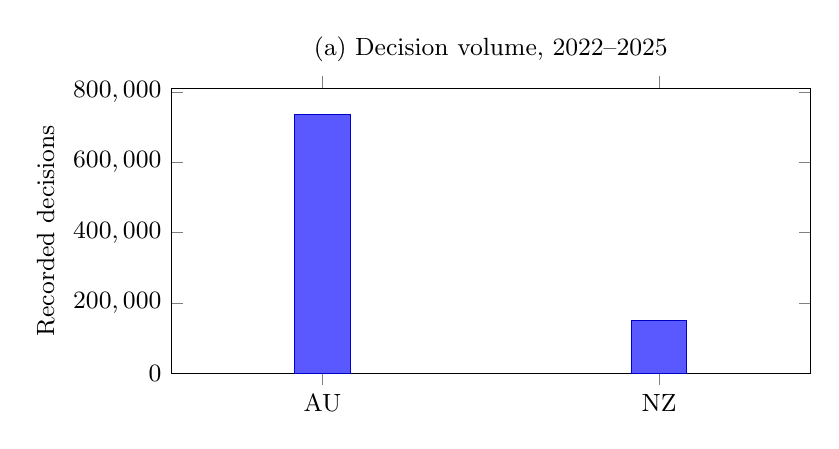
\begin{tikzpicture}
\begin{axis}[
  width=0.80\linewidth,
  height=5.2cm,
  ybar,
  bar width=20pt,
  symbolic x coords={AU,NZ},
  xtick=data,
  ymin=0,
  ylabel={Recorded decisions},
  title={(a) Decision volume, 2022--2025},
  scaled y ticks=false,
  yticklabel style={/pgf/number format/fixed,/pgf/number format/1000 sep={,}},
  enlarge x limits=0.45,
  tick label style={font=\small},
  label style={font=\small},
  title style={font=\small},
]
\addplot[fill=blue!65, draw=blue!80!black] coordinates {(AU,737424) (NZ,148746)};
\end{axis}
\end{tikzpicture}
\end{minipage}%
\hfill
\begin{minipage}[t]{0.46\textwidth}
\centering
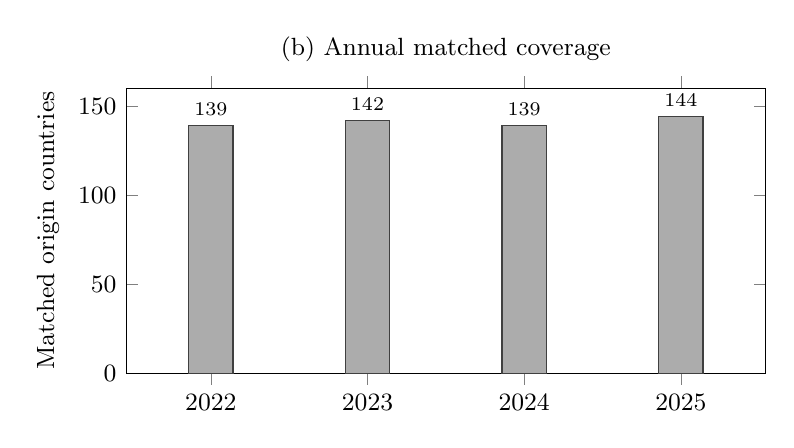
\begin{tikzpicture}
\begin{axis}[
  width=0.80\linewidth,
  height=5.2cm,
  ybar,
  bar width=16pt,
  symbolic x coords={2022,2023,2024,2025},
  xtick=data,
  ymin=0,
  ymax=160,
  ylabel={Matched origin countries},
  title={(b) Annual matched coverage},
  nodes near coords,
  every node near coord/.append style={font=\scriptsize},
  enlarge x limits=0.18,
  tick label style={font=\small},
  label style={font=\small},
  title style={font=\small},
]
\addplot[fill=gray!65, draw=black!75] coordinates {(2022,139) (2023,142) (2024,139) (2025,144)};
\end{axis}
\end{tikzpicture}
\end{minipage}

\caption{Scale and annual overlap of the validated comparison data. Panel (a) reports recorded two-outcome decisions pooled across 2022--2025. Panel (b) reports normalized origin countries represented in both destinations in each calendar year.}
\label{fig:data-coverage-overview}
\end{figure}

Table~\ref{tab:comparability-coverage} gives the pooled and annual overlap. The matched share was 87.4\% in the pooled data and ranged from 78.0\% to 79.9\% annually.

% Generated by scripts/generate_article_comparability_outputs.py. Do not edit.
\begin{table}
\caption{Observed origin-country overlap used by the comparability gate}
\label{tab:comparability-coverage}
\centering
\small
\begin{tabular}{lrrrrrr}
\toprule
Period & Union & Matched & Unmatched & AU only & NZ only & Matched share \\
\midrule
Pooled & 198 & 173 & 25 & 19 & 6 & 87.4\% \\
2022 & 174 & 139 & 35 & 25 & 10 & 79.9\% \\
2023 & 182 & 142 & 40 & 25 & 15 & 78.0\% \\
2024 & 174 & 139 & 35 & 23 & 12 & 79.9\% \\
2025 & 182 & 144 & 38 & 27 & 11 & 79.1\% \\
\bottomrule
\end{tabular}
\parbox{0.94\textwidth}{\scriptsize Notes: Union is the number of distinct origins observed in at least one destination. Matched origins are observed in both destinations with positive decision totals. Unmatched origins are retained for destination-specific analyses but excluded from paired analyses. They are not assigned zero decisions in the absent destination.}
\end{table}


Figure~\ref{fig:comparability-audit} separates the matched and destination-specific origins. The unmatched origins show why absence from one dataset cannot be interpreted as zero decisions.

\begin{figure}[H]
\centering
% Generated by scripts/generate_article_comparability_outputs.py. Do not edit.
\resizebox{\textwidth}{!}{%
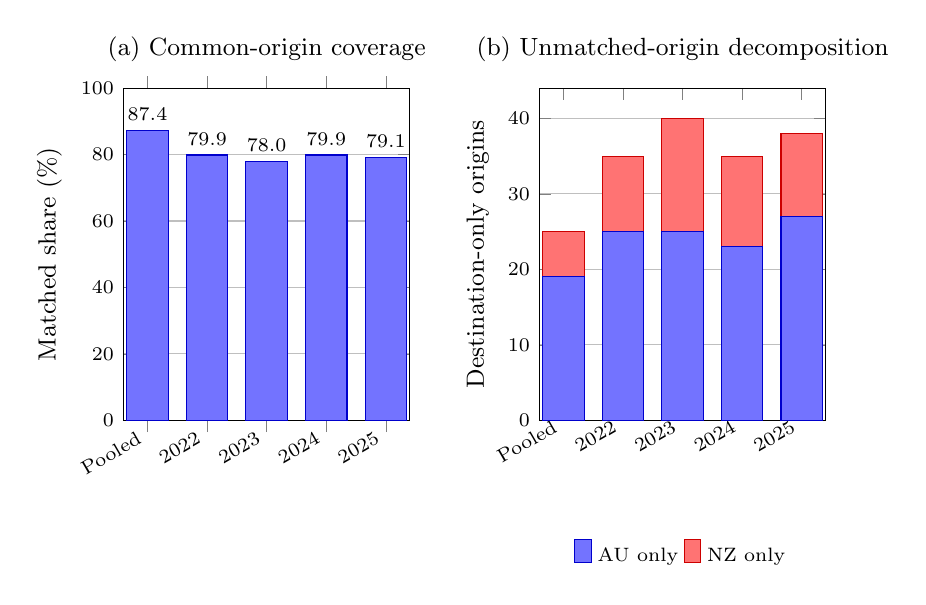
\begin{tikzpicture}
\begin{groupplot}[
  group style={group size=2 by 1,horizontal sep=1.65cm},
  width=0.43\textwidth,height=5.8cm,
  symbolic x coords={Pooled,2022,2023,2024,2025},xtick=data,
  tick label style={font=\scriptsize},label style={font=\small},title style={font=\small},
  x tick label style={rotate=30,anchor=east},ymajorgrids=true,
]
\nextgroupplot[ybar,bar width=15pt,ymin=0,ymax=100,ylabel={Matched share (\%)},title={(a) Common-origin coverage},nodes near coords,nodes near coords style={font=\scriptsize,/pgf/number format/fixed,/pgf/number format/fixed zerofill,/pgf/number format/precision=1}]
\addplot[fill=blue!55,draw=blue!80!black] coordinates {(Pooled,87.3737373737) (2022,79.8850574713) (2023,78.021978022) (2024,79.8850574713) (2025,79.1208791209)};
\nextgroupplot[ybar stacked,bar width=15pt,ymin=0,ylabel={Destination-only origins},title={(b) Unmatched-origin decomposition},legend columns=2,legend style={font=\scriptsize,draw=none,at={(0.5,-0.34)},anchor=north}]
\addplot[fill=blue!55,draw=blue!80!black] coordinates {(Pooled,19) (2022,25) (2023,25) (2024,23) (2025,27)};\addlegendentry{AU only}
\addplot[fill=red!55,draw=red!80!black] coordinates {(Pooled,6) (2022,10) (2023,15) (2024,12) (2025,11)};\addlegendentry{NZ only}
\end{groupplot}
\end{tikzpicture}%
}

\caption{Comparability audit for pooled and annual origin-country coverage. Panel (a) shows the share of origins in each observed union that occurred in both destinations. Panel (b) decomposes unmatched origins by the destination in which they were observed. Absence from the other destination was not treated as a zero count.}
\label{fig:comparability-audit}
\end{figure}

The subsequent paired analyses and pooled country-fixed-effect model therefore use the 173 origins observed in both destinations. Destination-only origins remain available for destination-specific descriptions but are not assigned zero decisions in the other destination.

\subsection{Destination Scale and Country-Level Distributions}

The first research question asks how the scale and approval structure differ between the two destinations. As shown in Table~\ref{tab:descriptive-comparison}, the decision-weighted aggregate approval rate was 86.7\% for Australia and 81.3\% for New Zealand. The Australian dataset also contained almost five times as many recorded decisions. These aggregate rates describe different sets and volumes of origin countries, so they do not establish that one destination is generally easier for an otherwise comparable applicant.

% Generated by scripts/generate_article_analysis_outputs.py. Do not edit.
\begin{table}
\caption{Descriptive comparison of destination-level and country-level outcomes, 2022--2025}
\label{tab:descriptive-comparison}
\centering
\small
Panel A: Decision-weighted destination summaries\par\smallskip
\begin{tabular}{l|rrr}
\toprule
Destination & Origins & Decisions & Aggregate approval (\%) \\
\midrule
Australia & 192 & 737,424 & 86.7 \\
New Zealand & 179 & 148,746 & 81.3 \\
\bottomrule
\end{tabular}

\medskip
Panel B: Country-weighted distributions\par\smallskip
\begin{tabular}{l|rr|rr}
\toprule
Statistic & AU approval (\%) & NZ approval (\%) & AU decisions & NZ decisions \\
\midrule
Minimum & 0.0 & 0.0 & 1 & 1 \\
First quartile & 83.8 & 54.4 & 7 & 5 \\
Median & 96.8 & 82.7 & 30.5 & 27 \\
Third quartile & 100.0 & 98.3 & 447.8 & 261.5 \\
Maximum & 100.0 & 100.0 & 236,751 & 35,472 \\
Mean & 88.4 & 71.9 & 3,840.8 & 831.0 \\
Standard deviation & 19.0 & 30.9 & 22,142.8 & 3,617.0 \\
Interquartile range & 16.2 & 43.9 & 440.8 & 256.5 \\
\bottomrule
\end{tabular}
\end{table}


The country-weighted distributions also differed. The median country approval rate was 96.8\% in Australia, with an interquartile range from 83.8\% to 100.0\%. The New Zealand median was 82.7\%, with an interquartile range from 54.4\% to 98.3\%. Median country decision volumes were similar at 30.5 decisions in Australia and 27 in New Zealand, but the upper quartiles were 447.8 and 261.5 decisions, respectively. These summaries show substantial variation between origin countries and strong right-skew in decision volume.

Figure~\ref{fig:decision-volume-log10-bins} groups origin countries by the order of magnitude of their recorded decision totals. Most origins had fewer than 100 decisions in each destination. Australia had more origins in the two largest volume groups, including two with at least 100,000 decisions, while New Zealand had none in that group.

\begin{figure}[H]
\centering
% Generated by scripts/generate_article_analysis_outputs.py. Do not edit.
\begin{minipage}[t]{0.48\textwidth}
\centering
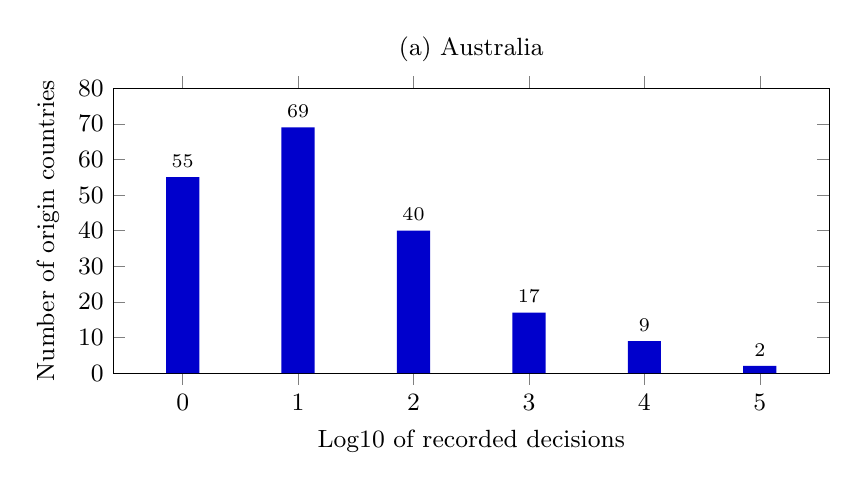
\begin{tikzpicture}
\begin{axis}[
  width=0.88\linewidth,
  height=5.2cm,
  xmin=-0.6, xmax=5.6, ymin=0, ymax=80,
  xtick={0,1,2,3,4,5}, ytick={0,10,...,80},
  xlabel={Log10 of recorded decisions}, ylabel={Number of origin countries},
  title={(a) Australia},
  ybar, bar width=12pt,
  nodes near coords,
  nodes near coords style={font=\scriptsize},
  tick label style={font=\small}, label style={font=\small}, title style={font=\small},
]
\addplot[fill=blue!80!black, draw=none] coordinates {(0,55) (1,69) (2,40) (3,17) (4,9) (5,2)};
\end{axis}
\end{tikzpicture}
\end{minipage}%
\hfill
\begin{minipage}[t]{0.48\textwidth}
\centering
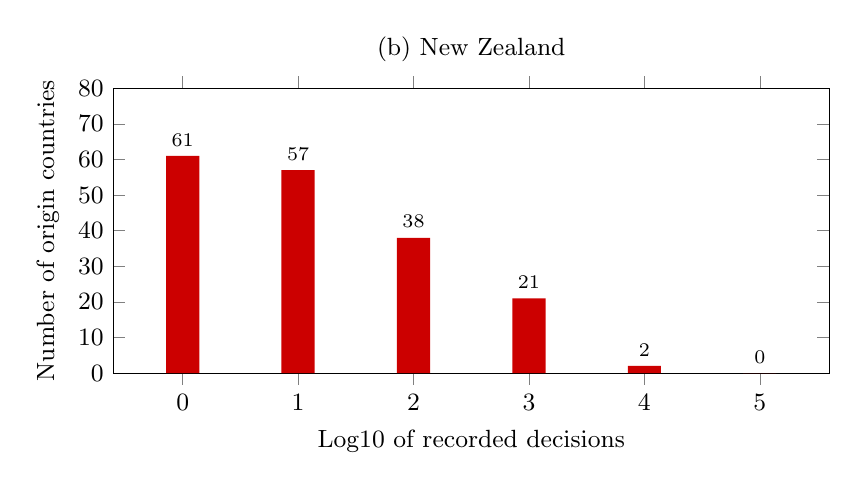
\begin{tikzpicture}
\begin{axis}[
  width=0.88\linewidth,
  height=5.2cm,
  xmin=-0.6, xmax=5.6, ymin=0, ymax=80,
  xtick={0,1,2,3,4,5}, ytick={0,10,...,80},
  xlabel={Log10 of recorded decisions}, ylabel={Number of origin countries},
  title={(b) New Zealand},
  ybar, bar width=12pt,
  nodes near coords,
  nodes near coords style={font=\scriptsize},
  tick label style={font=\small}, label style={font=\small}, title style={font=\small},
]
\addplot[fill=red!80!black, draw=none] coordinates {(0,61) (1,57) (2,38) (3,21) (4,2) (5,0)};
\end{axis}
\end{tikzpicture}
\end{minipage}

\caption{Distribution of pooled 2022--2025 recorded decision totals across represented origin countries, by destination. The x-axis is the integer part of the base-10 logarithm of each country's decision total: 0 represents 1--9 decisions, 1 represents 10--99, and so forth. Each represented origin contributes once within each destination.}
\label{fig:decision-volume-log10-bins}
\end{figure}

Figure~\ref{fig:descriptive-ecdfs} shows both empirical distributions. The Australian approval-rate curve lies mostly above the New Zealand curve, which is consistent with higher country-level rates across much of the distribution. The decision-volume curves show that most represented origins had relatively small counts in both destinations, while a limited number of origins accounted for very large volumes.

\begin{figure}[H]
\centering
% Generated by scripts/generate_article_analysis_outputs.py. Do not edit.
\begin{minipage}[t]{0.48\textwidth}
\centering
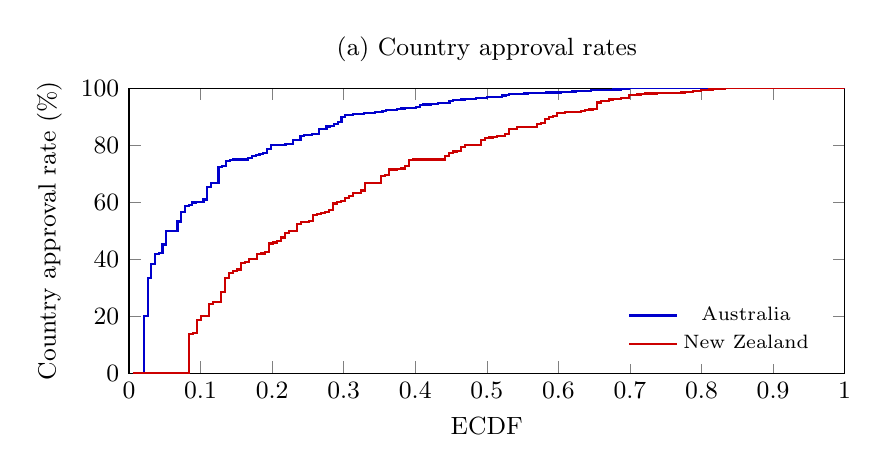
\begin{tikzpicture}
\begin{axis}[
  width=0.88\linewidth,
  height=5.2cm,
  xmin=0, xmax=1, ymin=0, ymax=100,
  xlabel={ECDF}, ylabel={Country approval rate (\%)},
  title={(a) Country approval rates},
  legend style={font=\scriptsize, at={(0.97,0.03)}, anchor=south east, draw=none},
  tick label style={font=\small}, label style={font=\small}, title style={font=\small},
]
\addplot[blue!80!black, thick, const plot] coordinates {(0.00520833333333,0) (0.0104166666667,0) (0.015625,0) (0.0208333333333,20) (0.0260416666667,33.3333333333) (0.03125,38.2352941176) (0.0364583333333,41.6666666667) (0.0416666666667,42.2222222222) (0.046875,45.1612903226) (0.0520833333333,50) (0.0572916666667,50) (0.0625,50) (0.0677083333333,53.2258064516) (0.0729166666667,56.6753135994) (0.078125,58.7012987013) (0.0833333333333,59.1111111111) (0.0885416666667,59.8976109215) (0.09375,60) (0.0989583333333,60) (0.104166666667,60.9189189189) (0.109375,65.3846153846) (0.114583333333,66.6666666667) (0.119791666667,66.6666666667) (0.125,72.3076923077) (0.130208333333,72.7272727273) (0.135416666667,74.420205671) (0.140625,74.9217659507) (0.145833333333,75) (0.151041666667,75) (0.15625,75) (0.161458333333,75) (0.166666666667,75.4098360656) (0.171875,76.1329305136) (0.177083333333,76.4705882353) (0.182291666667,76.9230769231) (0.1875,77.1428571429) (0.192708333333,78.6389413989) (0.197916666667,80) (0.203125,80) (0.208333333333,80) (0.213541666667,80.0875273523) (0.21875,80.309693971) (0.223958333333,80.4347826087) (0.229166666667,81.8181818182) (0.234375,81.8681318681) (0.239583333333,83.3333333333) (0.244791666667,83.5858585859) (0.25,83.7037037037) (0.255208333333,83.8709677419) (0.260416666667,83.9160839161) (0.265625,85.7142857143) (0.270833333333,85.7142857143) (0.276041666667,86.5588328576) (0.28125,86.7950481431) (0.286458333333,87.5) (0.291666666667,88.2352941176) (0.296875,90) (0.302083333333,90.4761904762) (0.307291666667,90.5405405405) (0.3125,90.8026755853) (0.317708333333,90.9090909091) (0.322916666667,90.9090909091) (0.328125,91.1964831804) (0.333333333333,91.3043478261) (0.338541666667,91.3043478261) (0.34375,91.6666666667) (0.348958333333,91.6666666667) (0.354166666667,91.935483871) (0.359375,92.2842933707) (0.364583333333,92.3694779116) (0.369791666667,92.4538040673) (0.375,92.6829268293) (0.380208333333,92.8571428571) (0.385416666667,93.056622216) (0.390625,93.1034482759) (0.395833333333,93.1623931624) (0.401041666667,93.3333333333) (0.40625,94.1994247363) (0.411458333333,94.2675159236) (0.416666666667,94.2857142857) (0.421875,94.3661971831) (0.427083333333,94.5544554455) (0.432291666667,94.7368421053) (0.4375,94.7570332481) (0.442708333333,94.9089949881) (0.447916666667,95.374800638) (0.453125,95.7142857143) (0.458333333333,95.8395245171) (0.463541666667,96) (0.46875,96.1538461538) (0.473958333333,96.1538461538) (0.479166666667,96.2848297214) (0.484375,96.6396292005) (0.489583333333,96.644295302) (0.494791666667,96.6666666667) (0.5,96.7741935484) (0.505208333333,96.875) (0.510416666667,96.9647435491) (0.515625,96.9954799256) (0.520833333333,97.4236641221) (0.526041666667,97.6) (0.53125,97.8431372549) (0.536458333333,97.8902953586) (0.541666666667,98) (0.546875,98.0198019802) (0.552083333333,98.1090100111) (0.557291666667,98.2229865291) (0.5625,98.2474226804) (0.567708333333,98.2876712329) (0.572916666667,98.3146067416) (0.578125,98.3311938383) (0.583333333333,98.4615384615) (0.588541666667,98.471659919) (0.59375,98.4799219639) (0.598958333333,98.4848484848) (0.604166666667,98.6590680523) (0.609375,98.7179487179) (0.614583333333,98.7864486769) (0.619791666667,98.8095238095) (0.625,98.8984384457) (0.630208333333,98.9130434783) (0.635416666667,98.9247311828) (0.640625,99.0040513167) (0.645833333333,99.299380221) (0.651041666667,99.3460678024) (0.65625,99.3630573248) (0.661458333333,99.3670886076) (0.666666666667,99.4758909853) (0.671875,99.4897959184) (0.677083333333,99.504950495) (0.682291666667,99.5449374289) (0.6875,99.6161898116) (0.692708333333,99.7101449275) (0.697916666667,100) (0.703125,100) (0.708333333333,100) (0.713541666667,100) (0.71875,100) (0.723958333333,100) (0.729166666667,100) (0.734375,100) (0.739583333333,100) (0.744791666667,100) (0.75,100) (0.755208333333,100) (0.760416666667,100) (0.765625,100) (0.770833333333,100) (0.776041666667,100) (0.78125,100) (0.786458333333,100) (0.791666666667,100) (0.796875,100) (0.802083333333,100) (0.807291666667,100) (0.8125,100) (0.817708333333,100) (0.822916666667,100) (0.828125,100) (0.833333333333,100) (0.838541666667,100) (0.84375,100) (0.848958333333,100) (0.854166666667,100) (0.859375,100) (0.864583333333,100) (0.869791666667,100) (0.875,100) (0.880208333333,100) (0.885416666667,100) (0.890625,100) (0.895833333333,100) (0.901041666667,100) (0.90625,100) (0.911458333333,100) (0.916666666667,100) (0.921875,100) (0.927083333333,100) (0.932291666667,100) (0.9375,100) (0.942708333333,100) (0.947916666667,100) (0.953125,100) (0.958333333333,100) (0.963541666667,100) (0.96875,100) (0.973958333333,100) (0.979166666667,100) (0.984375,100) (0.989583333333,100) (0.994791666667,100) (1,100)};
\addlegendentry{Australia}
\addplot[red!80!black, thick, const plot] coordinates {(0.00558659217877,0) (0.0111731843575,0) (0.0167597765363,0) (0.0223463687151,0) (0.0279329608939,0) (0.0335195530726,0) (0.0391061452514,0) (0.0446927374302,0) (0.0502793296089,0) (0.0558659217877,0) (0.0614525139665,0) (0.0670391061453,0) (0.072625698324,0) (0.0782122905028,0) (0.0837988826816,13.7931034483) (0.0893854748603,14.0845070423) (0.0949720670391,18.75) (0.100558659218,20) (0.106145251397,20) (0.111731843575,24.3243243243) (0.117318435754,25) (0.122905027933,25) (0.128491620112,28.5714285714) (0.134078212291,33.3333333333) (0.139664804469,35.2) (0.145251396648,35.7142857143) (0.150837988827,36.3636363636) (0.156424581006,38.7693572701) (0.162011173184,39.1241923905) (0.167597765363,40) (0.173184357542,40) (0.178770949721,41.6666666667) (0.184357541899,42) (0.189944134078,42.4242424242) (0.195530726257,45.4545454545) (0.201117318436,45.8333333333) (0.206703910615,46.4028776978) (0.212290502793,47.619047619) (0.217877094972,49.2560689115) (0.223463687151,50) (0.22905027933,50) (0.234636871508,52.380952381) (0.240223463687,52.9411764706) (0.245810055866,53.0546623794) (0.251396648045,53.3333333333) (0.256983240223,55.5555555556) (0.262569832402,55.751765893) (0.268156424581,56.1224489796) (0.27374301676,56.5621489123) (0.279329608939,57.1428571429) (0.284916201117,59.5238095238) (0.290502793296,60) (0.296089385475,60.4519774011) (0.301675977654,61.5384615385) (0.307262569832,62.1451104101) (0.312849162011,63.1578947368) (0.31843575419,63.179916318) (0.324022346369,64.1025641026) (0.329608938547,66.6666666667) (0.335195530726,66.6666666667) (0.340782122905,66.6666666667) (0.346368715084,66.6666666667) (0.351955307263,69.2628650904) (0.357541899441,69.5652173913) (0.36312849162,71.4285714286) (0.368715083799,71.4285714286) (0.374301675978,71.6417910448) (0.379888268156,71.7948717949) (0.385474860335,72.7272727273) (0.391061452514,74.8233782916) (0.396648044693,75) (0.402234636872,75) (0.40782122905,75) (0.413407821229,75) (0.418994413408,75) (0.424581005587,75) (0.430167597765,75) (0.435754189944,75) (0.441340782123,76.25) (0.446927374302,77.1929824561) (0.45251396648,77.7544596013) (0.458100558659,77.8846153846) (0.463687150838,79.4587945879) (0.469273743017,80) (0.474860335196,80) (0.480446927374,80) (0.486033519553,80) (0.491620111732,81.7531305903) (0.497206703911,82.6086956522) (0.502793296089,82.6923076923) (0.508379888268,82.7586206897) (0.513966480447,83.3333333333) (0.519553072626,83.3333333333) (0.525139664804,83.788791107) (0.530726256983,85.7142857143) (0.536312849162,85.8006042296) (0.541899441341,86.2676056338) (0.54748603352,86.3157894737) (0.553072625698,86.3636363636) (0.558659217877,86.4864864865) (0.564245810056,86.4864864865) (0.569832402235,87.5) (0.575418994413,87.8378378378) (0.581005586592,89.1704127503) (0.586592178771,90) (0.59217877095,90.1038062284) (0.597765363128,91.2087912088) (0.603351955307,91.3043478261) (0.608938547486,91.5721231767) (0.614525139665,91.6666666667) (0.620111731844,91.6666666667) (0.625698324022,91.6666666667) (0.631284916201,91.8918918919) (0.63687150838,92.3404255319) (0.642458100559,92.5416505231) (0.648044692737,92.7536231884) (0.653631284916,95.0105042017) (0.659217877095,95.4545454545) (0.664804469274,95.6204379562) (0.670391061453,96.0264900662) (0.675977653631,96.2962962963) (0.68156424581,96.3302752294) (0.687150837989,96.4370546318) (0.692737430168,96.6226883175) (0.698324022346,97.5782038345) (0.703910614525,97.6234003656) (0.709497206704,97.75390625) (0.715083798883,98.0434782609) (0.720670391061,98.1308411215) (0.72625698324,98.138869005) (0.731843575419,98.1481481481) (0.737430167598,98.2142857143) (0.743016759777,98.3009708738) (0.748603351955,98.3050847458) (0.754189944134,98.3563252128) (0.759776536313,98.4084880637) (0.765363128492,98.4195402299) (0.77094972067,98.4713076199) (0.776536312849,98.5714285714) (0.782122905028,98.75) (0.787709497207,98.9690721649) (0.793296089385,98.9898989899) (0.798882681564,99.4623655914) (0.804469273743,99.4993742178) (0.810055865922,99.564988136) (0.815642458101,99.6138996139) (0.821229050279,99.6875) (0.826815642458,99.7222222222) (0.832402234637,100) (0.837988826816,100) (0.843575418994,100) (0.849162011173,100) (0.854748603352,100) (0.860335195531,100) (0.865921787709,100) (0.871508379888,100) (0.877094972067,100) (0.882681564246,100) (0.888268156425,100) (0.893854748603,100) (0.899441340782,100) (0.905027932961,100) (0.91061452514,100) (0.916201117318,100) (0.921787709497,100) (0.927374301676,100) (0.932960893855,100) (0.938547486034,100) (0.944134078212,100) (0.949720670391,100) (0.95530726257,100) (0.960893854749,100) (0.966480446927,100) (0.972067039106,100) (0.977653631285,100) (0.983240223464,100) (0.988826815642,100) (0.994413407821,100) (1,100)};
\addlegendentry{New Zealand}
\end{axis}
\end{tikzpicture}
\end{minipage}%
\hfill
\begin{minipage}[t]{0.48\textwidth}
\centering
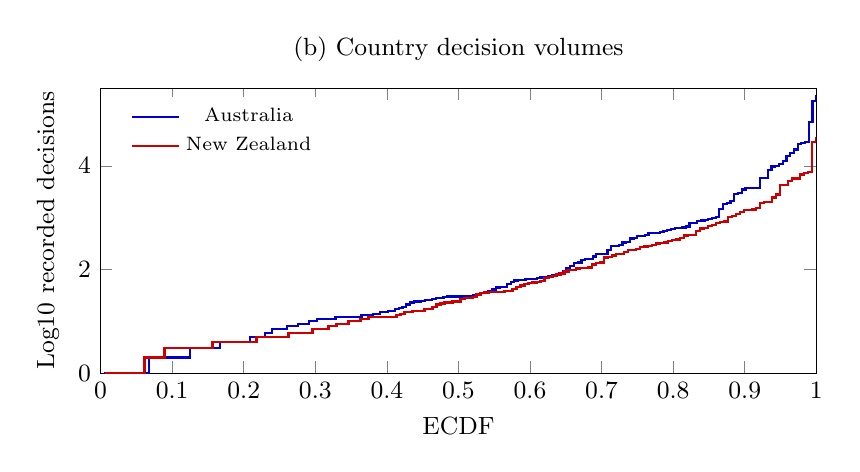
\begin{tikzpicture}
\begin{axis}[
  width=0.88\linewidth,
  height=5.2cm,
  xmin=0, xmax=1, ymin=0, ymax=5.5,
  xlabel={ECDF}, ylabel={Log10 recorded decisions},
  title={(b) Country decision volumes},
  legend style={font=\scriptsize, at={(0.03,0.97)}, anchor=north west, draw=none},
  tick label style={font=\small}, label style={font=\small}, title style={font=\small},
]
\addplot[blue!80!black, thick, const plot] coordinates {(0.00520833333333,0) (0.0104166666667,0) (0.015625,0) (0.0208333333333,0) (0.0260416666667,0) (0.03125,0) (0.0364583333333,0) (0.0416666666667,0) (0.046875,0) (0.0520833333333,0) (0.0572916666667,0) (0.0625,0) (0.0677083333333,0.301029995664) (0.0729166666667,0.301029995664) (0.078125,0.301029995664) (0.0833333333333,0.301029995664) (0.0885416666667,0.301029995664) (0.09375,0.301029995664) (0.0989583333333,0.301029995664) (0.104166666667,0.301029995664) (0.109375,0.301029995664) (0.114583333333,0.301029995664) (0.119791666667,0.301029995664) (0.125,0.47712125472) (0.130208333333,0.47712125472) (0.135416666667,0.47712125472) (0.140625,0.47712125472) (0.145833333333,0.47712125472) (0.151041666667,0.47712125472) (0.15625,0.47712125472) (0.161458333333,0.47712125472) (0.166666666667,0.602059991328) (0.171875,0.602059991328) (0.177083333333,0.602059991328) (0.182291666667,0.602059991328) (0.1875,0.602059991328) (0.192708333333,0.602059991328) (0.197916666667,0.602059991328) (0.203125,0.602059991328) (0.208333333333,0.698970004336) (0.213541666667,0.698970004336) (0.21875,0.698970004336) (0.223958333333,0.698970004336) (0.229166666667,0.778151250384) (0.234375,0.778151250384) (0.239583333333,0.845098040014) (0.244791666667,0.845098040014) (0.25,0.845098040014) (0.255208333333,0.845098040014) (0.260416666667,0.903089986992) (0.265625,0.903089986992) (0.270833333333,0.903089986992) (0.276041666667,0.954242509439) (0.28125,0.954242509439) (0.286458333333,0.954242509439) (0.291666666667,1) (0.296875,1) (0.302083333333,1.04139268516) (0.307291666667,1.04139268516) (0.3125,1.04139268516) (0.317708333333,1.04139268516) (0.322916666667,1.04139268516) (0.328125,1.07918124605) (0.333333333333,1.07918124605) (0.338541666667,1.07918124605) (0.34375,1.07918124605) (0.348958333333,1.07918124605) (0.354166666667,1.07918124605) (0.359375,1.07918124605) (0.364583333333,1.11394335231) (0.369791666667,1.11394335231) (0.375,1.11394335231) (0.380208333333,1.14612803568) (0.385416666667,1.14612803568) (0.390625,1.17609125906) (0.395833333333,1.17609125906) (0.401041666667,1.20411998266) (0.40625,1.20411998266) (0.411458333333,1.23044892138) (0.416666666667,1.2552725051) (0.421875,1.27875360095) (0.427083333333,1.32221929473) (0.432291666667,1.36172783602) (0.4375,1.38021124171) (0.442708333333,1.38021124171) (0.447916666667,1.39794000867) (0.453125,1.41497334797) (0.458333333333,1.41497334797) (0.463541666667,1.43136376416) (0.46875,1.44715803134) (0.473958333333,1.44715803134) (0.479166666667,1.4623979979) (0.484375,1.47712125472) (0.489583333333,1.47712125472) (0.494791666667,1.47712125472) (0.5,1.47712125472) (0.505208333333,1.49136169383) (0.510416666667,1.49136169383) (0.515625,1.49136169383) (0.520833333333,1.50514997832) (0.526041666667,1.53147891704) (0.53125,1.54406804435) (0.536458333333,1.55630250077) (0.541666666667,1.59106460703) (0.546875,1.61278385672) (0.552083333333,1.65321251378) (0.557291666667,1.66275783168) (0.5625,1.66275783168) (0.567708333333,1.71600334363) (0.572916666667,1.76342799356) (0.578125,1.78532983501) (0.583333333333,1.7923916895) (0.588541666667,1.7923916895) (0.59375,1.81291335664) (0.598958333333,1.81291335664) (0.604166666667,1.81954393554) (0.609375,1.83250891271) (0.614583333333,1.84509804001) (0.619791666667,1.85125834872) (0.625,1.86923171973) (0.630208333333,1.89209460269) (0.635416666667,1.89762709129) (0.640625,1.92427928606) (0.645833333333,1.96378782735) (0.651041666667,2.02118929907) (0.65625,2.06818586175) (0.661458333333,2.1303337685) (0.666666666667,2.13353890837) (0.671875,2.17609125906) (0.677083333333,2.19589965241) (0.682291666667,2.19865708695) (0.6875,2.25042000231) (0.692708333333,2.29225607136) (0.697916666667,2.30535136945) (0.703125,2.30535136945) (0.708333333333,2.37474834601) (0.713541666667,2.45484486001) (0.71875,2.45636603313) (0.723958333333,2.46538285145) (0.729166666667,2.51982799378) (0.734375,2.53781909507) (0.739583333333,2.59769518593) (0.744791666667,2.60638136511) (0.75,2.65030752313) (0.755208333333,2.65321251378) (0.760416666667,2.65991620007) (0.765625,2.69722934276) (0.770833333333,2.69897000434) (0.776041666667,2.7075701761) (0.78125,2.72345567204) (0.786458333333,2.74663419894) (0.791666666667,2.76789761602) (0.796875,2.77670118399) (0.802083333333,2.79726754083) (0.807291666667,2.79795964374) (0.8125,2.810232518) (0.817708333333,2.82801506422) (0.822916666667,2.89153745767) (0.828125,2.89320675306) (0.833333333333,2.93601079572) (0.838541666667,2.94398887507) (0.84375,2.95375969173) (0.848958333333,2.9795483747) (0.854166666667,2.98677173427) (0.859375,3.02036128265) (0.864583333333,3.16256440652) (0.869791666667,3.26007138799) (0.875,3.28443073384) (0.880208333333,3.31931430409) (0.885416666667,3.45727618606) (0.890625,3.47465325336) (0.895833333333,3.54270096945) (0.901041666667,3.56820172407) (0.90625,3.56949095435) (0.911458333333,3.57530333342) (0.916666666667,3.57875378443) (0.921875,3.76425087544) (0.927083333333,3.77261504985) (0.932291666667,3.91703262216) (0.9375,3.98618929974) (0.942708333333,3.99475694459) (0.947916666667,4.03798394945) (0.953125,4.08997572269) (0.958333333333,4.19769397508) (0.963541666667,4.25039560306) (0.96875,4.31620106867) (0.973958333333,4.41763773965) (0.979166666667,4.44933952617) (0.984375,4.45706398759) (0.989583333333,4.84337606541) (0.994791666667,5.24961899109) (1,5.37429182207)};
\addlegendentry{Australia}
\addplot[red!80!black, thick, const plot] coordinates {(0.00558659217877,0) (0.0111731843575,0) (0.0167597765363,0) (0.0223463687151,0) (0.0279329608939,0) (0.0335195530726,0) (0.0391061452514,0) (0.0446927374302,0) (0.0502793296089,0) (0.0558659217877,0) (0.0614525139665,0.301029995664) (0.0670391061453,0.301029995664) (0.072625698324,0.301029995664) (0.0782122905028,0.301029995664) (0.0837988826816,0.301029995664) (0.0893854748603,0.47712125472) (0.0949720670391,0.47712125472) (0.100558659218,0.47712125472) (0.106145251397,0.47712125472) (0.111731843575,0.47712125472) (0.117318435754,0.47712125472) (0.122905027933,0.47712125472) (0.128491620112,0.47712125472) (0.134078212291,0.47712125472) (0.139664804469,0.47712125472) (0.145251396648,0.47712125472) (0.150837988827,0.47712125472) (0.156424581006,0.602059991328) (0.162011173184,0.602059991328) (0.167597765363,0.602059991328) (0.173184357542,0.602059991328) (0.178770949721,0.602059991328) (0.184357541899,0.602059991328) (0.189944134078,0.602059991328) (0.195530726257,0.602059991328) (0.201117318436,0.602059991328) (0.206703910615,0.602059991328) (0.212290502793,0.602059991328) (0.217877094972,0.698970004336) (0.223463687151,0.698970004336) (0.22905027933,0.698970004336) (0.234636871508,0.698970004336) (0.240223463687,0.698970004336) (0.245810055866,0.698970004336) (0.251396648045,0.698970004336) (0.256983240223,0.698970004336) (0.262569832402,0.778151250384) (0.268156424581,0.778151250384) (0.27374301676,0.778151250384) (0.279329608939,0.778151250384) (0.284916201117,0.778151250384) (0.290502793296,0.778151250384) (0.296089385475,0.845098040014) (0.301675977654,0.845098040014) (0.307262569832,0.845098040014) (0.312849162011,0.845098040014) (0.31843575419,0.903089986992) (0.324022346369,0.903089986992) (0.329608938547,0.954242509439) (0.335195530726,0.954242509439) (0.340782122905,0.954242509439) (0.346368715084,1) (0.351955307263,1) (0.357541899441,1) (0.36312849162,1.04139268516) (0.368715083799,1.04139268516) (0.374301675978,1.07918124605) (0.379888268156,1.07918124605) (0.385474860335,1.07918124605) (0.391061452514,1.07918124605) (0.396648044693,1.07918124605) (0.402234636872,1.07918124605) (0.40782122905,1.07918124605) (0.413407821229,1.11394335231) (0.418994413408,1.14612803568) (0.424581005587,1.17609125906) (0.430167597765,1.17609125906) (0.435754189944,1.20411998266) (0.441340782123,1.20411998266) (0.446927374302,1.20411998266) (0.45251396648,1.23044892138) (0.458100558659,1.23044892138) (0.463687150838,1.27875360095) (0.469273743017,1.32221929473) (0.474860335196,1.34242268082) (0.480446927374,1.36172783602) (0.486033519553,1.36172783602) (0.491620111732,1.38021124171) (0.497206703911,1.38021124171) (0.502793296089,1.43136376416) (0.508379888268,1.44715803134) (0.513966480447,1.44715803134) (0.519553072626,1.4623979979) (0.525139664804,1.51851393988) (0.530726256983,1.54406804435) (0.536312849162,1.55630250077) (0.541899441341,1.56820172407) (0.54748603352,1.56820172407) (0.553072625698,1.56820172407) (0.558659217877,1.56820172407) (0.564245810056,1.59106460703) (0.569832402235,1.59106460703) (0.575418994413,1.6232492904) (0.581005586592,1.66275783168) (0.586592178771,1.69019608003) (0.59217877095,1.71600334363) (0.597765363128,1.73239375982) (0.603351955307,1.74818802701) (0.608938547486,1.76342799356) (0.614525139665,1.77085201164) (0.620111731844,1.83884909074) (0.625698324022,1.85125834872) (0.631284916201,1.86923171973) (0.63687150838,1.90308998699) (0.642458100559,1.92427928606) (0.648044692737,1.95904139232) (0.653631284916,1.98677173427) (0.659217877095,1.99122607569) (0.664804469274,2.0170333393) (0.670391061453,2.02938377769) (0.675977653631,2.03342375549) (0.68156424581,2.03742649794) (0.687150837989,2.09691001301) (0.692737430168,2.12057393121) (0.698324022346,2.13672056716) (0.703910614525,2.23299611039) (0.709497206704,2.24797326636) (0.715083798883,2.26951294422) (0.720670391061,2.29666519026) (0.72625698324,2.30319605742) (0.731843575419,2.33243845992) (0.737430167598,2.37839790095) (0.743016759777,2.38021124171) (0.748603351955,2.40140054078) (0.754189944134,2.43296929087) (0.759776536313,2.44404479592) (0.765363128492,2.45331834005) (0.77094972067,2.47275644932) (0.776536312849,2.50105926222) (0.782122905028,2.50514997832) (0.787709497207,2.51982799378) (0.793296089385,2.55630250077) (0.798882681564,2.57634135021) (0.804469273743,2.57978359662) (0.810055865922,2.61489721603) (0.815642458101,2.65609820201) (0.821229050279,2.66275783168) (0.826815642458,2.67209785794) (0.832402234637,2.74036268949) (0.837988826816,2.79028516403) (0.843575418994,2.79379038469) (0.849162011173,2.84260923961) (0.854748603352,2.85672889038) (0.860335195531,2.90254677931) (0.865921787709,2.91009054559) (0.871508379888,2.9253120915) (0.877094972067,3.01029995664) (0.882681564246,3.039017322) (0.888268156425,3.07554696139) (0.893854748603,3.10619089726) (0.899441340782,3.14395111642) (0.905027932961,3.14519640611) (0.91061452514,3.15986784709) (0.916201117318,3.19228861257) (0.921787709497,3.27966694405) (0.927374301676,3.29710365015) (0.932960893855,3.29710365015) (0.938547486034,3.38863396935) (0.944134078212,3.44638181222) (0.949720670391,3.62859325585) (0.95530726257,3.635282638) (0.960893854749,3.71281800021) (0.966480446927,3.7557224449) (0.972067039106,3.75724415102) (0.977653631285,3.83340212923) (0.983240223464,3.86314434625) (0.988826815642,3.88001283837) (0.994413407821,4.46794830529) (1,4.54988567577)};
\addlegendentry{New Zealand}
\end{axis}
\end{tikzpicture}
\end{minipage}

\caption{Country-level empirical cumulative distributions by destination. Panel (a) reports decision approval rates. Panel (b) reports recorded decision totals on a base-10 logarithmic scale. Each represented origin country contributes one observation.}
\label{fig:descriptive-ecdfs}
\end{figure}

\subsection{Matched-Country Approval-Rate Differences}

The second research question concerns the direction and magnitude of rate differences among matched countries. Among the 173 matched countries, the Australian rate was higher for 122 countries, the New Zealand rate was higher for 32, and the rates were equal for 19. The mean AU-minus-NZ difference was 16.32 percentage points (95\% CI 12.71, 19.93). The median difference was 9.44 percentage points (bootstrap 95\% CI 4.33, 14.53), as shown in Table~\ref{tab:matched-country-comparison}.

% Generated by scripts/generate_article_analysis_outputs.py. Do not edit.
\begin{table}
\caption{Matched-country AU-minus-NZ approval-rate comparison, 2022--2025}
\label{tab:matched-country-comparison}
\centering
\small
\begin{tabular}{lr}
\toprule
Quantity & Result \\
\midrule
Matched countries & 173 \\
AU higher / NZ higher / equal & 122 / 32 / 19 \\
Mean difference, percentage points (95\% CI) & 16.32 (12.71, 19.93) \\
Median difference, percentage points (bootstrap 95\% CI) & 9.44 (4.33, 14.53) \\
Standard deviation, percentage points & 24.05 \\
First / third quartile, percentage points & 0.00 / 25.96 \\
Range, percentage points & -25.00 to 100.00 \\
Wilcoxon signed-rank, $W$ ($n=154$) & 1419.5; $p<0.001$ \\
Paired $t$ sensitivity, $t(172)$ & 8.93; $p<0.001$ \\
\bottomrule
\end{tabular}
\end{table}


After removing the 19 exact zero differences, the two-sided Wilcoxon signed-rank test used 154 pairs. The smaller signed-rank sum was $W=1419.5$, with $p<0.001$. The paired $t$-test gave $t(172)=8.93$ and $p<0.001$. The primary test and the sensitivity test therefore both support a positive country-weighted AU-minus-NZ difference in this matched population.

\begin{figure}[!t]
\centering
% Generated by scripts/generate_article_analysis_outputs.py. Do not edit.
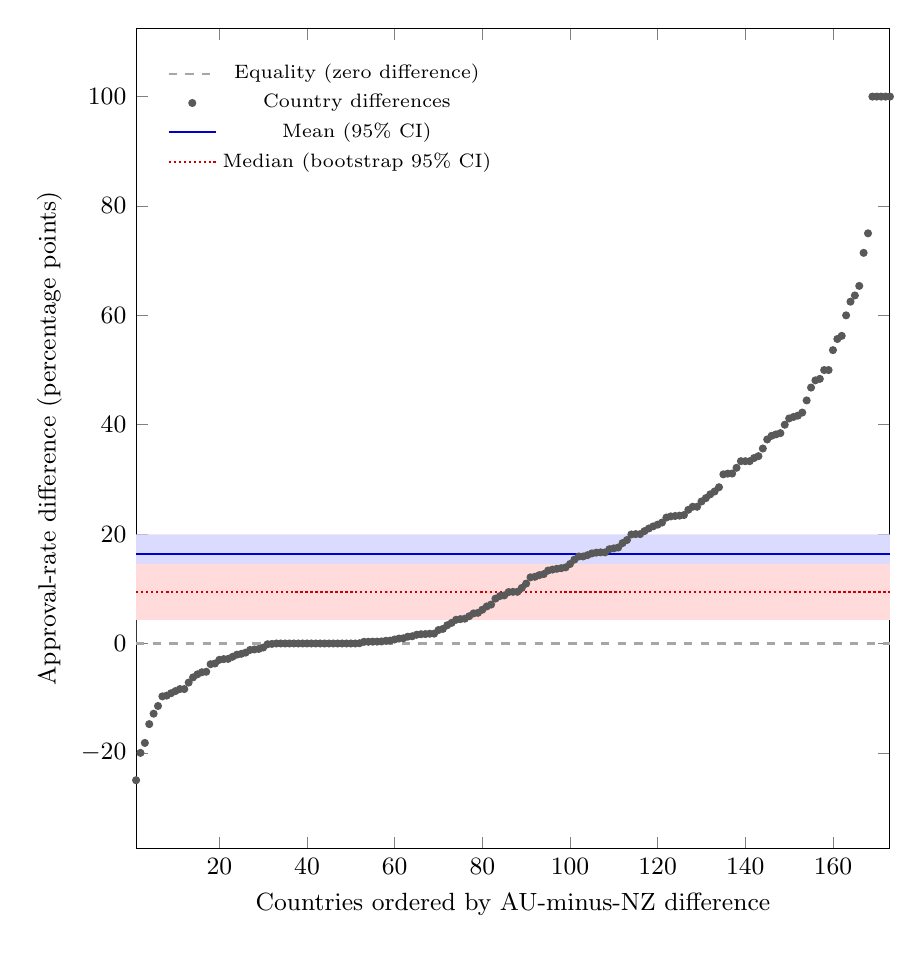
\begin{tikzpicture}
\begin{axis}[
  width=0.92\textwidth,
  height=12.0cm,
  xmin=1, xmax=173,
  xlabel={Countries ordered by AU-minus-NZ difference},
  ylabel={Approval-rate difference (percentage points)},
  legend style={font=\scriptsize, at={(0.03,0.97)}, anchor=north west, draw=none, fill=white},
  tick label style={font=\small}, label style={font=\small},
]
\addplot[draw=none, fill=blue!14, forget plot] coordinates {(1,12.7127171068) (173,12.7127171068) (173,19.9297411184) (1,19.9297411184)} \closedcycle;
\addplot[draw=none, fill=red!14, forget plot] coordinates {(1,4.33333333333) (173,4.33333333333) (173,14.5298337694) (1,14.5298337694)} \closedcycle;
\addplot[gray!70, dashed, thick, domain=1:173] {0};
\addlegendentry{Equality (zero difference)}
\addplot[only marks, mark=*, mark size=1.25pt, black!65] coordinates {(1,-25) (2,-20) (3,-18.1818181818) (4,-14.7435897436) (5,-12.8378378378) (6,-11.4285714286) (7,-9.6676064698) (8,-9.52380952381) (9,-9.09090909091) (10,-8.69565217391) (11,-8.33333333333) (12,-8.33333333333) (13,-7.14285714286) (14,-6.19535725053) (15,-5.6338028169) (16,-5.26315789474) (17,-5.16776677668) (18,-3.78787878788) (19,-3.65701215458) (20,-2.98245614035) (21,-2.85507891576) (22,-2.8152260111) (23,-2.43386243386) (24,-2.04456094364) (25,-1.89098998888) (26,-1.66666666667) (27,-1.19047619048) (28,-1.08695652174) (29,-0.995876107748) (30,-0.744416873449) (31,-0.138008628575) (32,-0.0772942254063) (33,0) (34,0) (35,0) (36,0) (37,0) (38,0) (39,0) (40,0) (41,0) (42,0) (43,0) (44,0) (45,0) (46,0) (47,0) (48,0) (49,0) (50,0) (51,0) (52,0.051201675544) (53,0.302742839499) (54,0.3125) (55,0.332790914018) (56,0.342055231583) (57,0.373158334942) (58,0.493516430412) (59,0.532743696734) (60,0.727951649536) (61,0.901718129398) (62,0.960144927536) (63,1.24396655511) (64,1.32361034673) (65,1.59399906235) (66,1.69491525424) (67,1.72266743681) (68,1.78571428571) (69,1.79910044978) (70,2.46138381388) (71,2.66723327667) (72,3.33687181147) (73,3.77594447521) (74,4.33333333333) (75,4.4538294025) (76,4.53506995148) (77,4.98310810811) (78,5.50271172299) (79,5.60675883257) (80,6.17110799439) (81,6.77419354839) (82,7.11441697106) (83,8.20512820513) (84,8.66501296031) (85,8.79120879121) (86,9.40114426668) (87,9.44335259009) (88,9.44522978979) (89,10.153142714) (90,10.9523809524) (91,12.0979020979) (92,12.1993957704) (93,12.5) (94,12.6829268293) (95,13.3333333333) (96,13.5135135135) (97,13.6565656566) (98,13.768115942) (99,13.9194139194) (100,14.5298337694) (101,15.3274942879) (102,15.9090909091) (103,15.91600605) (104,16.1538461538) (105,16.4705882353) (106,16.6091209898) (107,16.6666666667) (108,16.6666666667) (109,17.2413793103) (110,17.3913043478) (111,17.5511212089) (112,18.3596170385) (113,18.9189189189) (114,19.9336549565) (115,20) (116,20) (117,20.5458089669) (118,21.030004073) (119,21.416154467) (120,21.7338217338) (121,22.1153846154) (122,23.0288836846) (123,23.2397959184) (124,23.3146067416) (125,23.3789165396) (126,23.4848484848) (127,24.4421906694) (128,25) (129,25) (130,25.9582089552) (131,26.5766594267) (132,27.2727272727) (133,27.7936349365) (134,28.5714285714) (135,30.9297912713) (136,31.0606060606) (137,31.0767832803) (138,32.1224055135) (139,33.3333333333) (140,33.3333333333) (141,33.3333333333) (142,33.9068162732) (143,34.254194019) (144,35.6508484009) (145,37.304856323) (146,37.9710144928) (147,38.2352941176) (148,38.4615384615) (149,40) (150,41.1447623569) (151,41.4285714286) (152,41.6666666667) (153,42.2222222222) (154,44.4444444444) (155,46.7950481431) (156,48.1162981163) (157,48.3858585859) (158,50) (159,50) (160,53.6389413989) (161,55.6756756757) (162,56.25) (163,60) (164,62.5) (165,63.6363636364) (166,65.3846153846) (167,71.4285714286) (168,75) (169,100) (170,100) (171,100) (172,100) (173,100)};
\addlegendentry{Country differences}
\addplot[blue!80!black, thick, domain=1:173] {16.3212291126};
\addlegendentry{Mean (95\% CI)}
\addplot[red!80!black, thick, densely dotted, domain=1:173] {9.44335259009};
\addlegendentry{Median (bootstrap 95\% CI)}
\end{axis}
\end{tikzpicture}

\caption{Ordered country-level differences in approval rates for 173 origins represented in both destinations, with the mean and median differences and their 95\% confidence intervals. Differences are Australia minus New Zealand in percentage points. The gray dashed line marks equality. The blue band is the Student-$t$ interval for the mean, and the red band is the percentile-bootstrap interval for the median. These bands describe uncertainty in the summary estimates rather than the distribution of individual country differences.}
\label{fig:matched-difference-distribution}
\end{figure}

The ordered differences in Figure~\ref{fig:matched-difference-distribution} also show substantial heterogeneity. Some countries had higher rates in New Zealand, while the largest positive differences approached 100 percentage points. The overall positive result therefore does not imply a common difference for every origin. Small-denominator and threshold sensitivity analyses remain necessary before interpreting the most extreme country values.

\subsection{Cross-Destination Concordance}

The third research question asks whether countries with higher rates in one destination also tend to have higher rates in the other. Both measures showed positive association (Table~\ref{tab:approval-rate-concordance}). Pearson correlation was 0.629 (95\% CI 0.529 to 0.711, $p<0.001$), while Spearman rank correlation was 0.472 (bootstrap 95\% CI 0.320 to 0.609, $p<0.001$). Thus, the broad country patterns moved together, but the weaker rank correlation and the dispersion in Figure~\ref{fig:approval-rate-concordance} show that country positions were not identical.

% Generated by scripts/generate_article_concordance_country_outputs.py. Do not edit.
\begin{table}
\caption{Cross-destination concordance of matched-country approval rates, 2022--2025}
\label{tab:approval-rate-concordance}
\centering
\small
\begin{tabular}{lrrrr}
\toprule
Method & Coefficient & 95\% CI & $n$ & Two-sided $p$ \\
\midrule
Pearson & 0.629 & (0.529, 0.711) & 173 & $p<0.001$ \\
Spearman & 0.472 & (0.320, 0.609) & 173 & $p<0.001$ \\
\bottomrule
\end{tabular}
\end{table}


\begin{figure}[H]
\centering
% Generated by scripts/generate_article_concordance_country_outputs.py. Do not edit.
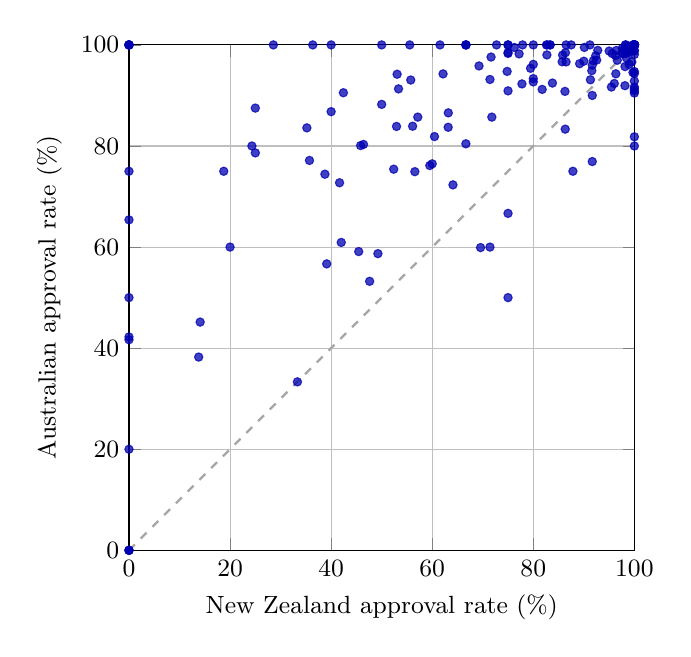
\begin{tikzpicture}
\begin{axis}[
  width=0.78\textwidth, height=8.0cm,
  xmin=0, xmax=100, ymin=0, ymax=100,
  xlabel={New Zealand approval rate (\%)}, ylabel={Australian approval rate (\%)},
  axis equal image, grid=major, tick label style={font=\small}, label style={font=\small},
]
\addplot[gray!70, dashed, thick, domain=0:100] {x};
\addplot[only marks, mark=*, mark size=1.5pt, blue!70!black, opacity=0.75] coordinates {(14.08450704,45.16129032) (71.42857143,60) (41.66666667,72.72727273) (0,100) (85.80060423,98) (50,88.23529412) (100,98.91304348) (80,92.68292683) (100,100) (100,94.73684211) (55.75176589,93.05662222) (100,100) (75,90.90909091) (99.46236559,98.71794872) (100,100) (28.57142857,100) (50,100) (63.17991632,86.55883286) (82.60869565,100) (100,100) (75,98.31460674) (89.17041275,96.28482972) (100,100) (83.33333333,100) (0,65.38461538) (100,100) (91.57212318,94.90899499) (13.79310345,38.23529412) (98.57142857,99.29938022) (0,75) (90.10380623,99.5049505) (96.62268832,96.96474355) (98.13886901,98.47165992) (92.75362319,98.92473118) (74.82337829,94.75703325) (0,0) (87.5,100) (100,80) (98.96907216,96.15384615) (0,100) (18.75,75) (99.6875,100) (0,100) (66.66666667,100) (61.53846154,100) (71.42857143,93.16239316) (56.12244898,83.91608392) (100,92.85714286) (75,66.66666667) (100,90.90909091) (80,100) (64.1025641,72.30769231) (79.45879459,95.37480064) (91.20879121,100) (97.75390625,98.24742268) (57.14285714,85.71428571) (99.61389961,99.47589099) (45.45454545,59.11111111) (91.66666667,96) (75,100) (75,98.48484848) (0,100) (83.33333333,100) (20,60) (72.72727273,100) (98.21428571,100) (100,100) (56.56214891,74.92176595) (95.0105042,98.78644868) (53.05466238,94.19942474) (47.61904762,53.22580645) (98.13084112,91.93548387) (86.48648649,100) (99.49937422,96.6442953) (91.66666667,90) (99.56498814,99.61618981) (59.52380952,76.13293051) (76.25,99.48979592) (46.4028777,80.30969397) (77.88461538,100) (98.40848806,98.33119384) (66.66666667,80.43478261) (96.02649007,92.36947791) (91.66666667,76.92307692) (69.56521739,59.89761092) (0,41.66666667) (36.36363636,100) (100,100) (90,96.77419355) (100,91.66666667) (0,50) (60,76.47058824) (97.57820383,98.47992196) (82.69230769,98.01980198) (75,50) (100,81.81818182) (100,100) (86.48648649,96.6396292) (92.34042553,97.84313725) (100,100) (60.4519774,81.86813187) (52.94117647,83.87096774) (80,96.15384615) (49.25606891,58.7012987) (55.55555556,100) (100,100) (38.76935727,74.42020567) (98.98989899,99.36305732) (100,100) (0,100) (42,60.91891892) (100,94.36619718) (98.30097087,99.54493743) (95.62043796,98.28767123) (39.12419239,56.6753136) (91.89189189,96.875) (86.26760563,90.80267559) (86.36363636,98.46153846) (71.64179104,97.6) (83.78879111,92.45380407) (100,98.80952381) (96.2962963,97.89029536) (98.47130762,99.00405132) (91.30434783,93.10344828) (69.26286509,95.83952452) (52.38095238,75.40983607) (66.66666667,100) (100,100) (95.45454545,91.66666667) (77.19298246,98.22298653) (0,0) (75,100) (100,90.47619048) (0,42.22222222) (96.43705463,98.89843845) (100,91.30434783) (100,100) (96.33027523,94.28571429) (0,20) (62.14511041,94.26751592) (33.33333333,33.33333333) (99.72222222,94.55445545) (77.7544596,92.28429337) (53.33333333,91.30434783) (35.71428571,77.14285714) (100,100) (98.75,99.71014493) (98.04347826,99.36708861) (24.32432432,80) (97.62340037,99.3460678) (66.66666667,100) (92.54165052,96.99547993) (98.14814815,95.71428571) (0,0) (86.31578947,83.33333333) (80,93.33333333) (40,100) (98.30508475,100) (35.2,83.58585859) (45.83333333,80.08752735) (85.71428571,96.66666667) (100,98.10901001) (98.41954023,97.42366412) (42.42424242,90.54054054) (98.35632521,98.65906805) (82.75862069,100) (25,78.6389414) (87.83783784,75) (71.79487179,85.71428571) (81.75313059,91.19648318) (25,87.5) (63.15789474,83.7037037) (40,86.79504814)};
\end{axis}
\end{tikzpicture}

\caption{Australian and New Zealand approval rates for 173 matched origin countries. Both axes use the same scale. The dashed equality line indicates equal rates and is not a fitted model.}
\label{fig:approval-rate-concordance}
\end{figure}

These coefficients do not imply agreement. Many observations lie above or below the equality line, and the matched-country analysis found a positive average AU-minus-NZ difference. The results therefore answer the ordering question: higher-rate countries in Australia generally also tended to have higher rates in New Zealand. They do not show that the two destinations assigned the same rates to those countries.

\subsection{Country-Specific Differences}

The fourth research question asks which individual origins show evidence of a destination difference. Of the 173 country comparisons, 60 met the expected-count rule for Pearson's chi-square test and 113 used Fisher's exact test. After Benjamini--Hochberg correction across all 173 tests, 56 remained significant at the 0.05 false-discovery-rate threshold. The direction counts were unchanged from the paired analysis: Australia had the higher observed rate for 122 countries, New Zealand for 32, and 19 were equal. Zero cells required the declared correction for supplementary risk-ratio and odds-ratio estimates in 65 comparisons.

Table~\ref{tab:country-specific-results} gives the ten largest absolute differences within the forest-plot population. All ten shown differences were positive and remained significant after adjustment. The largest displayed difference was 48.4 percentage points for Türkiye, followed by 46.8 points for Zimbabwe and 41.1 points for Iran (Islamic Republic of). These are country-level aggregate comparisons and must not be read as causal effects on otherwise identical individual applicants.

% Generated by scripts/generate_article_concordance_country_outputs.py. Do not edit.
\begin{table}[H]
\caption{Largest displayed country-specific AU-minus-NZ differences among countries with at least 50 decisions in each destination}
\label{tab:country-specific-results}
\centering
\scriptsize
\begin{tabular}{lrrrl}
\toprule
Country & AU $n$ & NZ $n$ & Difference, pp (95\% CI) & BH $q$ \\
\midrule
Türkiye & 396 & 125 & 48.4 (38.8, 56.9) & $<0.001$ \\
Zimbabwe & 1,454 & 215 & 46.8 (39.9, 53.3) & $<0.001$ \\
Iran (Islamic Republic of) & 2,086 & 622 & 41.1 (37.1, 45.2) & $<0.001$ \\
Bangladesh & 28,646 & 1,982 & 37.3 (35.1, 39.5) & $<0.001$ \\
Nepal & 69,723 & 7,297 & 35.7 (34.5, 36.8) & $<0.001$ \\
Kenya & 10,914 & 278 & 33.9 (28.0, 39.7) & $<0.001$ \\
South Africa & 628 & 317 & 32.1 (26.5, 37.8) & $<0.001$ \\
Egypt & 286 & 98 & 27.8 (17.3, 38.4) & $<0.001$ \\
Russian Federation & 673 & 719 & 26.6 (22.9, 30.3) & $<0.001$ \\
Peru & 500 & 201 & 26.0 (19.9, 32.6) & $<0.001$ \\
\bottomrule
\end{tabular}
\parbox{0.94\textwidth}{\scriptsize Notes: The complete table contains all 173 matched countries. Difference is Australia minus New Zealand. BH denotes the Benjamini--Hochberg adjusted $q$-value.}
\end{table}


\begin{figure}[H]
\centering
% Generated by scripts/generate_article_concordance_country_outputs.py. Do not edit.
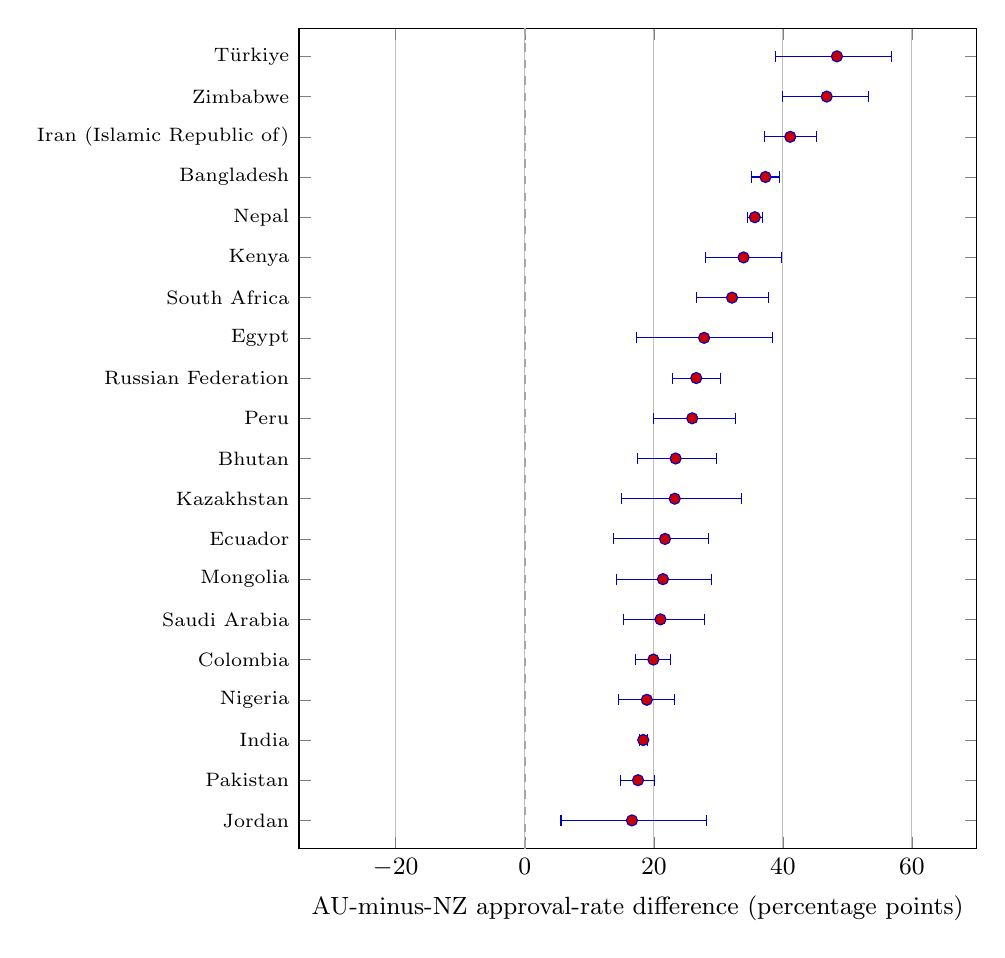
\begin{tikzpicture}
\begin{axis}[
  width=0.84\textwidth, height=12.0cm,
  xmin=-35, xmax=70, ymin=0.3, ymax=20.7,
  xlabel={AU-minus-NZ approval-rate difference (percentage points)},
  ytick={1,2,3,4,5,6,7,8,9,10,11,12,13,14,15,16,17,18,19,20}, yticklabels={{Jordan},{Pakistan},{India},{Nigeria},{Colombia},{Saudi Arabia},{Mongolia},{Ecuador},{Kazakhstan},{Bhutan},{Peru},{Russian Federation},{Egypt},{South Africa},{Kenya},{Nepal},{Bangladesh},{Iran (Islamic Republic of)},{Zimbabwe},{Türkiye}},
  y tick label style={font=\scriptsize}, tick label style={font=\small}, label style={font=\small},
  xmajorgrids=true,
]
\addplot[gray!70, dashed, thick, domain=0.3:20.7] (0,x);
\addplot+[only marks, mark=*, blue!75!black, error bars/.cd, x dir=both, x explicit] coordinates {(16.60912099,1) += (11.51301076,0) -= (10.99645407,0) (17.55112121,2) += (2.594752254,0) -= (2.653499461,0) (18.35961704,3) += (0.6022141601,0) -= (0.6009582004,0) (18.91891892,4) += (4.345113207,0) -= (4.456861073,0) (19.93365496,5) += (2.596666475,0) -= (2.755625012,0) (21.03000407,6) += (6.85650276,0) -= (5.672164601,0) (21.41615447,7) += (7.546345555,0) -= (7.147763059,0) (21.73382173,8) += (6.747087898,0) -= (8.012941349,0) (23.23979592,9) += (10.39926715,0) -= (8.316278443,0) (23.37891654,10) += (6.300089722,0) -= (5.886264785,0) (25.95820896,11) += (6.670430425,0) -= (6.038433103,0) (26.57665943,12) += (3.691616035,0) -= (3.720054153,0) (27.79363494,13) += (10.57895175,0) -= (10.51933374,0) (32.12240551,14) += (5.674233194,0) -= (5.575078282,0) (33.90681627,15) += (5.820040324,0) -= (5.920012362,0) (35.6508484,16) += (1.157550832,0) -= (1.169651141,0) (37.30485632,17) += (2.214548422,0) -= (2.194037261,0) (41.14476236,18) += (4.03601757,0) -= (4.040167521,0) (46.79504814,19) += (6.527797662,0) -= (6.917095832,0) (48.38585859,20) += (8.493884775,0) -= (9.561766232,0)};
\end{axis}
\end{tikzpicture}

\caption{Selected country-specific AU-minus-NZ approval-rate differences with Newcombe 95\% confidence intervals. The plot shows the 20 largest absolute differences among countries with at least 50 decisions in each destination. The complete 173-country result is retained in the CSV artifact.}
\label{fig:country-difference-forest}
\end{figure}

The forest plot shows that substantial positive differences were present even after the denominator restriction used for display. It is not a sensitivity analysis: the selection rule affects presentation only, and all 173 countries were included in hypothesis testing and FDR adjustment. The planned threshold analysis remains necessary to determine whether broader conclusions change when countries with fewer than 20 or 50 decisions in either destination are excluded.

\subsection{Binomial Regression Results}

The fifth research question asks whether destination is associated with approval probability after accounting for origin-country differences. The pooled fixed-effect model retained 155 matched origins and 885,588 decisions after excluding 18 outcome-invariant countries. The Australian destination coefficient was 0.942 (cluster-robust SE 0.190), corresponding to an odds ratio of 2.57 (95\% CI 1.77 to 3.72, $p<0.001$). Standardized approval probabilities were 85.3\% for Australia and 74.4\% for New Zealand. Their adjusted contrast was 10.9 percentage points (95\% CI 6.6 to 15.2 points).

% Generated by scripts/generate_article_model_outputs.py. Do not edit.
\begin{table}
\caption{Pooled origin-adjusted destination association, 2022--2025}
\label{tab:pooled-binomial-regression}
\centering
\small
\begin{tabular}{lr}
\toprule
Quantity & Result \\
\midrule
Retained matched origins & 155 \\
Recorded decisions & 885,588 \\
Australian destination coefficient & 0.942 \\
Cluster-robust standard error & 0.190 \\
Odds ratio (95\% CI) & 2.57 (1.77, 3.72) \\
Standardized Australian probability, \% (95\% CI) & 85.3 (83.8, 86.8) \\
Standardized New Zealand probability, \% (95\% CI) & 74.4 (71.6, 77.2) \\
Adjusted AU-minus-NZ difference, pp (95\% CI) & 10.9 (6.6, 15.2) \\
Destination test & $p<0.001$ \\
\bottomrule
\end{tabular}
\parbox{0.94\textwidth}{\scriptsize Notes: New Zealand is the reference destination. The model uses origin-country fixed effects and country-cluster-robust CR1 standard errors. Standardized probabilities are averaged equally over the retained matched origins. CI denotes confidence interval and pp denotes percentage points.}
\end{table}


Figure~\ref{fig:pooled-standardized-probabilities} shows the standardized destination probabilities and their adjusted difference on the probability scale.

\begin{figure}[H]
\centering
% Generated by scripts/generate_article_model_outputs.py. Do not edit.
\begin{minipage}[t]{0.49\textwidth}
\centering
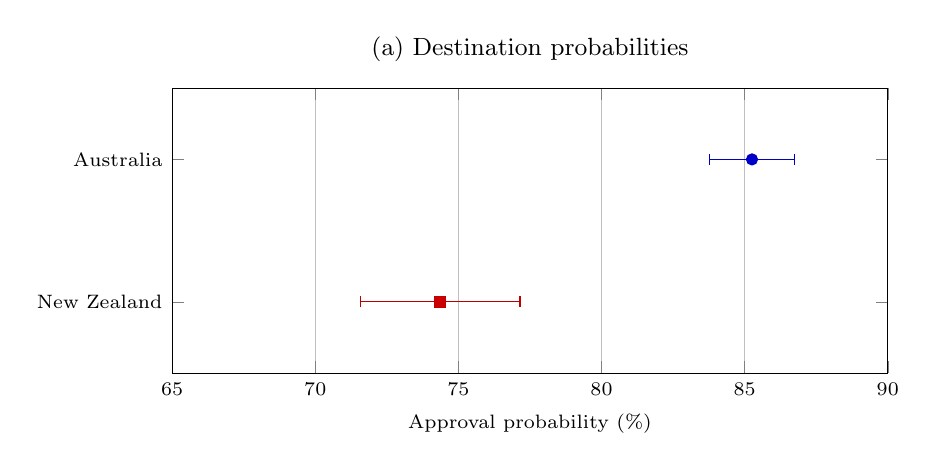
\begin{tikzpicture}
\begin{axis}[
  width=0.88\linewidth, height=5.2cm,
  xmin=65, xmax=90, ymin=0.5, ymax=2.5,
  xlabel={Approval probability (\%)},
  ytick={1,2}, yticklabels={{New Zealand},{Australia}},
  title={(a) Destination probabilities},
  xmajorgrids=true, tick label style={font=\scriptsize},
  label style={font=\scriptsize}, title style={font=\small},
]
\addplot+[only marks, mark=*, blue!75!black, error bars/.cd, x dir=both, x explicit]
  coordinates {(85.2563078057,2) += (1.49611928468,0) -= (1.49611928468,0)};
\addplot+[only marks, mark=square*, red!75!black, error bars/.cd, x dir=both, x explicit]
  coordinates {(74.3708141052,1) += (2.78200270637,0) -= (2.78200270637,0)};
\end{axis}
\end{tikzpicture}
\end{minipage}%
\hfill
\begin{minipage}[t]{0.49\textwidth}
\centering
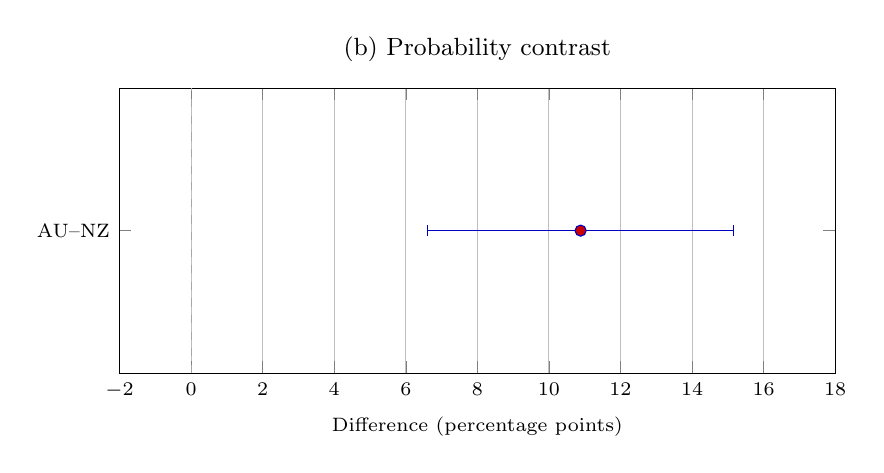
\begin{tikzpicture}
\begin{axis}[
  width=0.88\linewidth, height=5.2cm,
  xmin=-2, xmax=18, ymin=0.5, ymax=1.5,
  xlabel={Difference (percentage points)},
  ytick={1}, yticklabels={{AU--NZ}},
  title={(b) Probability contrast},
  xmajorgrids=true, tick label style={font=\scriptsize},
  label style={font=\scriptsize}, title style={font=\small},
]
\addplot[gray!70, dashed] coordinates {(0,0.5) (0,1.5)};
\addplot+[only marks, mark=*, blue!75!black, error bars/.cd, x dir=both, x explicit]
  coordinates {(10.8854937005,1) += (4.27812199105,0) -= (4.27812199105,0)};
\end{axis}
\end{tikzpicture}
\end{minipage}

\caption{Origin-adjusted approval probabilities and their Australian-minus-New Zealand contrast from the pooled country-fixed-effect binomial model. Points are standardized estimates and error bars are 95\% confidence intervals. Probabilities are averaged equally over the 155 retained matched origins.}
\label{fig:pooled-standardized-probabilities}
\end{figure}

The pooled model was computationally stable and was retained for estimating the average origin-adjusted association between destination and approval. It converged in six iterations, produced no fitting warnings, had finite coefficients and standard errors, and had no fitted probabilities beyond the declared extreme threshold. This stability does not mean that the model captured the country-specific variation well. The Pearson dispersion ratio was 22.66, far above the value of about 1 expected when ordinary binomial variation adequately describes the data \cite{Williams1982}. The largest Cook's distances \cite{Pregibon1981} occurred for the Australian observations for Bangladesh (42.70), Nepal (34.36), and China (17.88). These observations were retained. We therefore interpret the destination coefficient as an average association while reporting the substantial unexplained variation without applying a dispersion adjustment. The cluster-robust interval addresses within-origin dependence, but the estimate remains a conditional observational association and not a causal effect of destination choice.

\section{Robustness or Sensitivity Checks}

We checked whether the main findings changed when origins with few recorded decisions were excluded. At minimum thresholds of 20, 50, and 100 decisions in each destination, the Australian-minus-New Zealand differences remained positive and statistically significant. Approval-rate concordance became stronger after origins with small decision totals were removed.

The denominator restrictions reduced the matched population from 173 origins to 91 at a minimum of 20 decisions in each destination, 66 at a minimum of 50, and 54 at a minimum of 100 (Table~\ref{tab:sensitivity-paired}). The mean Australian-minus-New Zealand difference decreased from 16.3 percentage points for all matched origins to 11.9 points at the 20-decision threshold and 10.6 points at the 50-decision threshold, before increasing slightly to 11.3 points at the 100-decision threshold. The corresponding median differences were 9.4, 7.1, 5.0, and 5.0 points. Every mean and median interval remained above zero, and both the paired $t$ and Wilcoxon tests remained significant at each threshold.

% Generated by scripts/generate_article_sensitivity_outputs.py. Do not edit.
\begin{table}[H]
\caption{Sensitivity of paired differences to minimum decision denominators}
\label{tab:sensitivity-paired}
\centering
\small
\begin{tabular}{rrrrrr}
\toprule
Minimum & Origins & \shortstack{Mean difference, pp\\(95\% CI)} & \shortstack{Median difference, pp\\(95\% CI)} & \shortstack{AU\\decisions} & \shortstack{NZ\\decisions} \\
\midrule
0 & 173 & 16.3 (12.7, 19.9) & 9.4 (4.3, 14.5) & 737,336 & 148,726 \\
20 & 91 & 11.9 (8.7, 15.2) & 7.1 (2.7, 12.1) & 735,399 & 147,406 \\
50 & 66 & 10.6 (7.3, 13.9) & 5.0 (1.5, 10.8) & 731,427 & 146,489 \\
100 & 54 & 11.3 (7.5, 15.1) & 5.0 (1.5, 12.9) & 729,184 & 145,192 \\
\bottomrule
\end{tabular}
\parbox{0.94\textwidth}{\scriptsize Notes: Threshold 0 includes every pooled matched origin. All displayed mean and median intervals exclude zero. Differences are Australia minus New Zealand.}
\end{table}
\medskip
\begin{table}[H]
\caption{Sensitivity of approval-rate concordance to minimum decision denominators}
\label{tab:sensitivity-concordance}
\centering
\small
\begin{tabular*}{0.94\textwidth}{@{\extracolsep{\fill}}rrrr@{}}
\toprule
Minimum & Origins & Pearson $r$ (95\% CI) & Spearman $\rho$ (95\% CI) \\
\midrule
0 & 173 & 0.629 (0.529, 0.711) & 0.472 (0.320, 0.609) \\
20 & 91 & 0.778 (0.682, 0.848) & 0.739 (0.612, 0.825) \\
50 & 66 & 0.792 (0.681, 0.868) & 0.725 (0.558, 0.838) \\
100 & 54 & 0.794 (0.668, 0.876) & 0.815 (0.676, 0.900) \\
\bottomrule
\end{tabular*}
\parbox{0.94\textwidth}{\scriptsize Notes: All correlation intervals exclude zero.}
\end{table}


Approval-rate concordance became stronger after sparse origins were removed (Table~\ref{tab:sensitivity-concordance}). Pearson correlation increased from 0.629 for all 173 origins to 0.778, 0.792, and 0.794 at the 20-, 50-, and 100-decision thresholds, respectively. Spearman correlation increased from 0.472 to 0.739, 0.725, and 0.815. All correlation intervals excluded zero. The stronger restricted-sample correlations indicate that unstable rates among small-denominator origins weakened the complete-sample association, while the positive paired differences remained present in the restricted populations.

\begin{figure}[H]
\centering
% Generated by scripts/generate_article_sensitivity_outputs.py. Do not edit.
\begin{minipage}[t]{0.49\textwidth}
\centering
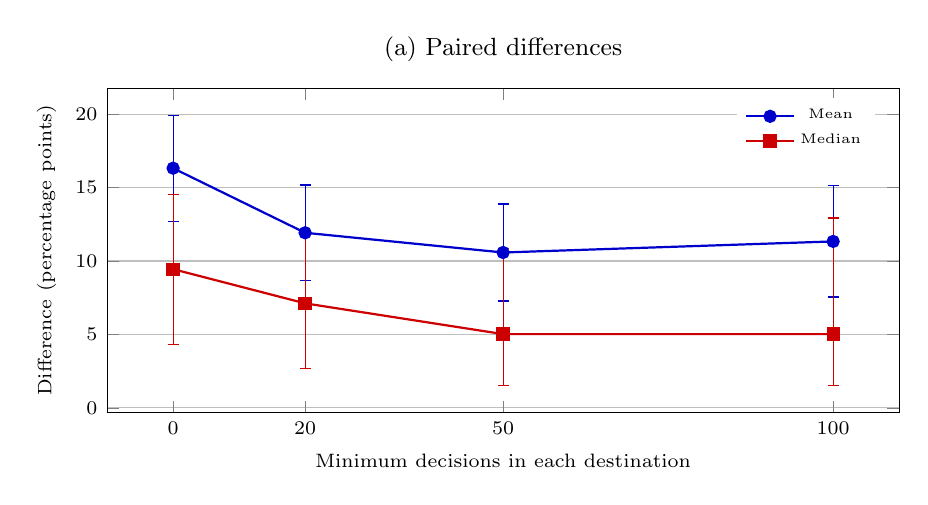
\begin{tikzpicture}
\begin{axis}[width=0.96\linewidth,height=5.7cm,xtick={0,20,50,100},xlabel={Minimum decisions in each destination},ylabel={Difference (percentage points)},title={(a) Paired differences},ymajorgrids=true,legend style={font=\tiny,draw=none,at={(0.97,0.97)},anchor=north east},label style={font=\scriptsize},title style={font=\small},tick label style={font=\scriptsize}]
\addplot+[blue!80!black,thick,mark=*,error bars/.cd,y dir=both,y explicit] coordinates {(0,16.3212291126) += (0,3.60851200581) -= (0,3.60851200581) (20,11.9214823092) += (0,3.2573172331) -= (0,3.2573172331) (50,10.5788998257) += (0,3.30406602317) -= (0,3.30406602317) (100,11.3325341779) += (0,3.78613946145) -= (0,3.78613946145)};\addlegendentry{Mean}
\addplot+[red!80!black,thick,mark=square*,error bars/.cd,y dir=both,y explicit] coordinates {(0,9.44335259009) += (0,5.08648117933) -= (0,5.11001925675) (20,7.11441697106) += (0,4.98348512685) -= (0,4.44718369438) (50,5.01889083723) += (0,5.80342194286) -= (0,3.49575194547) (100,5.01889083723) += (0,7.90908987624) -= (0,3.49575194547)};\addlegendentry{Median}
\end{axis}
\end{tikzpicture}
\end{minipage}%
\hfill
\begin{minipage}[t]{0.49\textwidth}
\centering
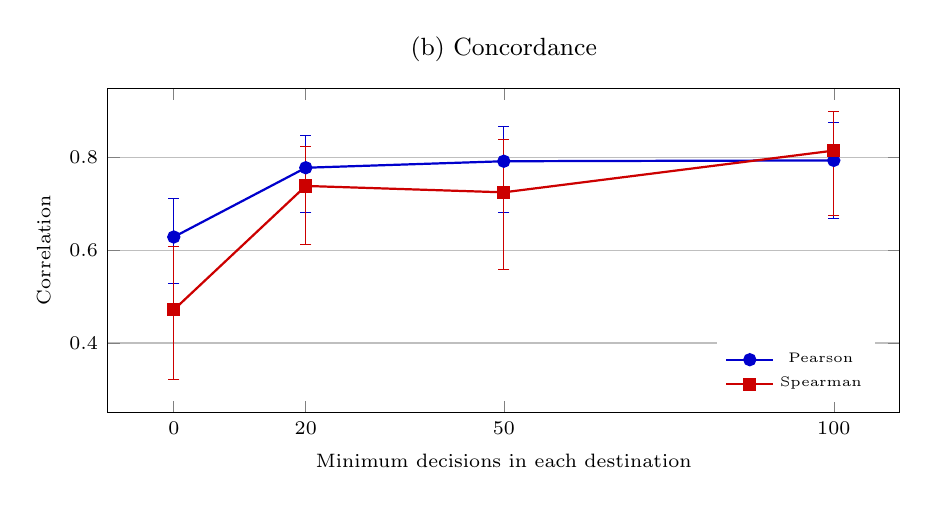
\begin{tikzpicture}
\begin{axis}[width=0.96\linewidth,height=5.7cm,xtick={0,20,50,100},xlabel={Minimum decisions in each destination},ylabel={Correlation},title={(b) Concordance},ymin=0.25,ymax=0.95,ymajorgrids=true,legend style={font=\tiny,draw=none,at={(0.97,0.03)},anchor=south east},label style={font=\scriptsize},title style={font=\small},tick label style={font=\scriptsize}]
\addplot+[blue!80!black,thick,mark=*,error bars/.cd,y dir=both,y explicit] coordinates {(0,0.628764936684) += (0,0.0824772757362) -= (0,0.0995539699297) (20,0.778255499572) += (0,0.0699900012082) -= (0,0.0967079704952) (50,0.792278284926) += (0,0.0756090351804) -= (0,0.111485846637) (100,0.794105075549) += (0,0.0815664948145) -= (0,0.125620714106)};\addlegendentry{Pearson}
\addplot+[red!80!black,thick,mark=square*,error bars/.cd,y dir=both,y explicit] coordinates {(0,0.471509609824) += (0,0.137626578282) -= (0,0.151165670113) (20,0.738964732893) += (0,0.0860524590963) -= (0,0.127167483926) (50,0.725171956745) += (0,0.113113366222) -= (0,0.166751999638) (100,0.815284924719) += (0,0.0849255224356) -= (0,0.139612652526)};\addlegendentry{Spearman}
\end{axis}
\end{tikzpicture}
\end{minipage}

\caption{Sensitivity to pre-specified minimum decision denominators in both destinations. Panel (a) shows country-weighted mean and median Australian-minus-New Zealand differences. Panel (b) shows Pearson and Spearman approval-rate concordance. Error bars are the corresponding 95\% intervals.}
\label{fig:threshold-sensitivity}
\end{figure}

\section{Discussion}

This study found a positive average Australian-minus-New Zealand difference under the study definitions, but not a uniform difference across origins. Among 173 matched applicant origins, the Australian decision approval rate was higher for 122 origins, the New Zealand rate was higher for 32, and the rates were equal for 19. The country-weighted mean difference was 16.3 percentage points. After accounting for origin-country differences in the pooled model, the standardized difference remained positive at 10.9 points. The direction also remained positive at every pre-specified minimum-decision threshold. Taken together, these results support an average destination-associated difference in the observed records while showing that its size depends on the analytical population and summary used.

The cross-destination concordance helps place this average difference in context. Origins with higher decision approval rates in one destination generally also tended to have higher rates in the other, which is consistent with applicant-origin context contributing to the observed pattern. Earlier modelling within New Zealand likewise found associations between approval rates and regional, economic, development, and health characteristics of applicant origins \cite{Kaplan2026NZVisaApproval}. The present comparison shows that origin context is not sufficient: statistically supported differences remain when the same published origin labels are compared across Australia and New Zealand. Approval rates are therefore better understood as outcomes associated with an origin--destination pair than as fixed attributes of either the origin or the destination alone.

The country-specific and model results show why the pair-based interpretation is necessary. Fifty-six origin-specific differences remained significant after adjustment for multiple testing, but their sizes and directions varied. The pooled model also had substantial overdispersion and influential observations, showing that origin fixed effects and one common destination coefficient did not describe all origin--destination variation. The smaller mean differences after sparse origins were excluded further show that the numerical size of the overall contrast depends partly on which origins are included. The pooled coefficient is therefore useful as a summary of the average conditional association, but it should not replace the country-specific results or be interpreted as the same difference for every origin.

This relational interpretation is consistent with research showing that international student mobility reflects characteristics of both origins and destinations \cite{PerkinsNeumayer2014,Weber2023}. It also accords with evidence that a destination-side visa reform can change applications and approval outcomes for selected origins \cite{Gonnot2025}. The present study adds a matched-origin comparison of recorded visa decisions, but it cannot identify the mechanism producing any particular difference. Applicant selection, visa-category coverage, evidentiary requirements, institutional composition, policy priorities, and administrative practice remain possible explanations rather than findings of this analysis.

The study also demonstrates a reproducible way to compare public visa statistics without treating unlike administrative totals as directly interchangeable. It defines the same recorded decision outcome in both sources, restricts paired analyses to origins observed in both destinations, preserves absent records as unobserved rather than assigning zeros, reports country-specific effects with multiple-testing control, and examines sensitivity to small decision totals. These choices reduce avoidable measurement and analytical errors, but they cannot make the two source populations identical or turn aggregate associations into individual or causal conclusions.

The next study should examine how applicant-origin composition, alternative weighting of national summaries, annual changes, and a country-and-year model affect the comparison. Further explanatory work should also add regional classifications and publicly available official country-level indicators, such as measures of income, development, health, and infrastructure, and test whether their associations differ between Australia and New Zealand. The earlier New Zealand results provide a basis for these extensions \cite{Kaplan2026NZVisaApproval}. Explaining policy mechanisms, however, will require directly comparable policy measures, applicant characteristics, or decision reasons rather than country-level associations alone.

\section{Limitations}

The main limitation is that the two official sources describe similar, but not identical, student visa populations. The New Zealand data include all published offshore or overseas student visa decision records used in this study. The more detailed Australian source allowed us to select primary applicants outside Australia in the Higher Education Sector as the closest available comparison. Matching origin-country names and calculating both rates from approvals or grants and declines or refusals make the sources more comparable, but differences in reporting structure and visa-category coverage remain. The calculated rates do not include withdrawals or other outcomes in their totals. The results therefore compare the closest populations available in the public data, not identical groups of applicants or visa categories.

The paired analyses are limited to the 173 origins with recorded decisions in both destinations. Twenty-five origins appeared in only one destination's pooled data and were excluded rather than treated as having zero decisions in the other destination. The pooled regression has a narrower scope because 18 origins with no variation in their recorded outcomes were excluded. Its standardized comparison consequently describes the 155 retained matched origins, weighted equally, rather than all origins in either source or the overall population of applicants.

The records are aggregated by applicant origin and do not contain individual characteristics, application evidence, institutional information, or reasons for decisions. The observed differences cannot identify why an application was approved or refused, distinguish applicant selection from destination policy or administrative practice, evaluate otherwise similar applicants, or estimate an individual's probability of approval. The findings are therefore aggregate associations and do not establish that a particular policy caused an origin-specific difference. Many origins also had small decision totals. The threshold checks showed that the overall direction was robust to excluding these origins, but estimates for individual small-denominator origins remain less stable.

Finally, pooling decisions from 2022--2025 describes an average comparison and can conceal changes between years. The substantial overdispersion and influential observations show that origin fixed effects and one common destination coefficient do not capture all variation between origin--destination pairs. Cluster-robust standard errors account for dependence within origins, but they do not explain that remaining heterogeneity or correct an incomplete model specification. Applicant-origin composition, alternative weighting of national summaries, annual changes, and country-and-year modelling are therefore outside the scope of this article.

\section{Conclusion}

This study compares student visa approval rates in Australia and New Zealand. It applies the same definition of a completed decision and matches applicant-origin countries across the two datasets. Under these definitions, the average Australian-minus-New Zealand difference is positive, but its magnitude varies across origins and analytical specifications. The persistence of the contrast after origins are matched and modelled shows that applicant origin alone is not sufficient to explain the observed rates.

This finding complements earlier New Zealand evidence that approval-rate variation within one destination is associated with regional, economic, development, and health characteristics of applicant origins \cite{Kaplan2026NZVisaApproval}. Together, the studies show that approval rates are neither simple attributes of origin countries nor context-free properties of destination countries. The same destination produces different rates across origins, while the same origin produces different rates across destinations. Explanation therefore requires the origin--destination pair: the interaction between an origin-specific applicant population and the way a destination's immigration system operates for that population.

This pair-based perspective directs further research towards visa-category design, evidentiary requirements, policy priorities, institutional settings, applicant selection, processing practices, and changes in migration or international-education strategy. The present aggregate data do not distinguish among these mechanisms or demonstrate that any named policy caused a particular difference. The next study should therefore examine pair-specific variation more directly, including the distribution of decision volumes across origins, alternative weighting of national summaries, changes across years, and a country-and-year fixed-effect binomial model of whether the adjusted destination association is stable over time.

\section{Appendices or Supplementary Material}

\subsection{Repository Structure}

% To be written if needed.

\subsection{Student Visa Application Preparation}

% To be written if needed.

\subsection{Countries Excluded Before Regression}

% To be written if needed.

\subsection{Full Correlation Table}

% To be written if needed.

\subsection{Coefficient Stability Summary}

% To be written if needed.

\subsection{Relative Residual Tables}

% To be written if needed.

\subsection{Prediction Table}

% To be written if needed.

\bibliographystyle{splncs04}
\bibliography{bibliography}

\end{document}
